% Options for packages loaded elsewhere
\PassOptionsToPackage{unicode}{hyperref}
\PassOptionsToPackage{hyphens}{url}
\PassOptionsToPackage{dvipsnames,svgnames,x11names}{xcolor}
%
\documentclass[
  12pt]{article}

\usepackage{amsmath,amssymb}
\usepackage{iftex}
\ifPDFTeX
  \usepackage[T1]{fontenc}
  \usepackage[utf8]{inputenc}
  \usepackage{textcomp} % provide euro and other symbols
\else % if luatex or xetex
  \usepackage{unicode-math}
  \defaultfontfeatures{Scale=MatchLowercase}
  \defaultfontfeatures[\rmfamily]{Ligatures=TeX,Scale=1}
\fi
\usepackage{lmodern}
\ifPDFTeX\else  
    % xetex/luatex font selection
\fi
% Use upquote if available, for straight quotes in verbatim environments
\IfFileExists{upquote.sty}{\usepackage{upquote}}{}
\IfFileExists{microtype.sty}{% use microtype if available
  \usepackage[]{microtype}
  \UseMicrotypeSet[protrusion]{basicmath} % disable protrusion for tt fonts
}{}
\makeatletter
\@ifundefined{KOMAClassName}{% if non-KOMA class
  \IfFileExists{parskip.sty}{%
    \usepackage{parskip}
  }{% else
    \setlength{\parindent}{0pt}
    \setlength{\parskip}{6pt plus 2pt minus 1pt}}
}{% if KOMA class
  \KOMAoptions{parskip=half}}
\makeatother
\usepackage{xcolor}
\setlength{\emergencystretch}{3em} % prevent overfull lines
\setcounter{secnumdepth}{5}
% Make \paragraph and \subparagraph free-standing
\ifx\paragraph\undefined\else
  \let\oldparagraph\paragraph
  \renewcommand{\paragraph}[1]{\oldparagraph{#1}\mbox{}}
\fi
\ifx\subparagraph\undefined\else
  \let\oldsubparagraph\subparagraph
  \renewcommand{\subparagraph}[1]{\oldsubparagraph{#1}\mbox{}}
\fi


\providecommand{\tightlist}{%
  \setlength{\itemsep}{0pt}\setlength{\parskip}{0pt}}\usepackage{longtable,booktabs,array}
\usepackage{calc} % for calculating minipage widths
% Correct order of tables after \paragraph or \subparagraph
\usepackage{etoolbox}
\makeatletter
\patchcmd\longtable{\par}{\if@noskipsec\mbox{}\fi\par}{}{}
\makeatother
% Allow footnotes in longtable head/foot
\IfFileExists{footnotehyper.sty}{\usepackage{footnotehyper}}{\usepackage{footnote}}
\makesavenoteenv{longtable}
\usepackage{graphicx}
\makeatletter
\def\maxwidth{\ifdim\Gin@nat@width>\linewidth\linewidth\else\Gin@nat@width\fi}
\def\maxheight{\ifdim\Gin@nat@height>\textheight\textheight\else\Gin@nat@height\fi}
\makeatother
% Scale images if necessary, so that they will not overflow the page
% margins by default, and it is still possible to overwrite the defaults
% using explicit options in \includegraphics[width, height, ...]{}
\setkeys{Gin}{width=\maxwidth,height=\maxheight,keepaspectratio}
% Set default figure placement to htbp
\makeatletter
\def\fps@figure{htbp}
\makeatother

\addtolength{\oddsidemargin}{-.5in}%
\addtolength{\evensidemargin}{-1in}%
\addtolength{\textwidth}{1in}%
\addtolength{\textheight}{1.7in}%
\addtolength{\topmargin}{-1in}%

\usepackage{amsthm}
\newtheorem{ass}{Assumption}
% \usepackage{mathtools}
\usepackage[final, nomargin, inline, nomarginclue, author=HM]{fixme}
% \fxusetargetlayout{color}
\fxsetface{inline}{\color{blue}}
\fxsetface{env}{\color{blue}}
% \usepackage{amsmath}
% \usepackage[final,nomargin,index,inline, author=]{fixme}
% \usepackage{bbm}
\usepackage{unicode-math}
\usepackage{tabularx}
\usepackage{adjustbox}
% \usepackage{amsmath}
% - \usepackage{longtable}
% - \usepackage{booktabs}
% - \usepackage{graphicx}
% \newtheorem{definition}{Definition}
% \newtheorem{theo}{Theorem}
% \newtheorem{lemma}{Lemma}
% \newtheorem{ass}{Assumption}
% \usepackage{xkvltxp}
% -  #final or draft
% - \fxsetup{envlayout=color, targetlayout=color}
% - \fxsetface{inline}{\color{blue}}

% kableExtra required packages:
\usepackage{booktabs}
\usepackage{longtable}
% \usepackage{array}
% \usepackage{multirow}
% \usepackage{wrapfig}
% \usepackage{float}
% \usepackage{colortbl}
% \usepackage{pdflscape}
% \usepackage{tabu}
\usepackage{threeparttable}
\usepackage{threeparttablex}
% \usepackage[normalem]{ulem}
% \usepackage{makecell}
% \usepackage{xcolor}
\usepackage{booktabs}
\usepackage{longtable}
\usepackage{array}
\usepackage{multirow}
\usepackage{wrapfig}
\usepackage{float}
\usepackage{colortbl}
\usepackage{pdflscape}
\usepackage{tabu}
\usepackage{threeparttable}
\usepackage{threeparttablex}
\usepackage[normalem]{ulem}
\usepackage{makecell}
\usepackage{xcolor}
\makeatletter
\@ifpackageloaded{caption}{}{\usepackage{caption}}
\AtBeginDocument{%
\ifdefined\contentsname
  \renewcommand*\contentsname{Table of contents}
\else
  \newcommand\contentsname{Table of contents}
\fi
\ifdefined\listfigurename
  \renewcommand*\listfigurename{List of Figures}
\else
  \newcommand\listfigurename{List of Figures}
\fi
\ifdefined\listtablename
  \renewcommand*\listtablename{List of Tables}
\else
  \newcommand\listtablename{List of Tables}
\fi
\ifdefined\figurename
  \renewcommand*\figurename{Figure}
\else
  \newcommand\figurename{Figure}
\fi
\ifdefined\tablename
  \renewcommand*\tablename{Table}
\else
  \newcommand\tablename{Table}
\fi
}
\@ifpackageloaded{float}{}{\usepackage{float}}
\floatstyle{ruled}
\@ifundefined{c@chapter}{\newfloat{codelisting}{h}{lop}}{\newfloat{codelisting}{h}{lop}[chapter]}
\floatname{codelisting}{Listing}
\newcommand*\listoflistings{\listof{codelisting}{List of Listings}}
\usepackage{amsthm}
\theoremstyle{definition}
\newtheorem{definition}{Definition}[section]
\theoremstyle{remark}
\AtBeginDocument{\renewcommand*{\proofname}{Proof}}
\newtheorem*{remark}{Remark}
\newtheorem*{solution}{Solution}
\newtheorem{refremark}{Remark}[section]
\newtheorem{refsolution}{Solution}[section]
\makeatother
\makeatletter
\makeatother
\makeatletter
\@ifpackageloaded{caption}{}{\usepackage{caption}}
\@ifpackageloaded{subcaption}{}{\usepackage{subcaption}}
\makeatother
\makeatletter
\@ifpackageloaded{tcolorbox}{}{\usepackage[many]{tcolorbox}}
\makeatother
%%%% ---foldboxy preamble ----- %%%%%

\definecolor{fbx-default-color1}{HTML}{c7c7d0}
\definecolor{fbx-default-color2}{HTML}{a3a3aa}

\definecolor{fbox-color1}{HTML}{c7c7d0}
\definecolor{fbox-color2}{HTML}{a3a3aa}

% arguments: #1 typelabelnummer: #2 titel: #3
\newenvironment{fbx}[3]{\begin{tcolorbox}[enhanced, breakable,%
attach boxed title to top*={xshift=1.4pt},
boxed title style={boxrule=0.0mm, fuzzy shadow={1pt}{-1pt}{0mm}{0.1mm}{gray}, arc=.3em, rounded corners=east, sharp corners=west}, colframe=#1-color2, colbacktitle=#1-color1, colback = white, coltitle=black,  titlerule=0mm, toprule=0pt, bottomrule=.7pt, leftrule=.3em, rightrule=0pt, outer arc=.3em,  arc=0pt,	 sharp corners = east, left=.5em, bottomtitle=1mm, toptitle=1mm,title=\textbf{#2}\hspace{0.5em}{#3}]}
{\end{tcolorbox}}

% boxed environment with right border
\newenvironment{fbxSimple}[3]{\begin{tcolorbox}[enhanced, breakable,%
attach boxed title to top*={xshift=1.4pt},
boxed title style={boxrule=0.0mm, fuzzy shadow={1pt}{-1pt}{0mm}{0.1mm}{gray}, arc=.3em, rounded corners=east, sharp corners=west}, colframe=#1-color2, colbacktitle=#1-color1, colback = white, coltitle=black,  titlerule=0mm, toprule=0pt, bottomrule=.7pt, leftrule=.3em, rightrule=.7pt, outer arc=.3em,  	left=.5em, right=.5em, bottomtitle=1mm, toptitle=1mm,title=\textbf{#2}\hspace{0.5em}{#3}]}
{\end{tcolorbox}}

%%%% --- end foldboxy preamble ----- %%%%%
%%==== colors from yaml ===%
\definecolor{Theorem-color1}{HTML}{99CCFF}
\definecolor{Theorem-color2}{HTML}{FFFFFF}
\definecolor{Definition-color1}{HTML}{99CCFF}
\definecolor{Definition-color2}{HTML}{FFFFFF}
\definecolor{Proposition-color1}{HTML}{99CCFF}
\definecolor{Proposition-color2}{HTML}{FFFFFF}
\definecolor{Assumption-color1}{HTML}{99CCFF}
\definecolor{Assumption-color2}{HTML}{FFFFFF}
%=============%
\ifLuaTeX
  \usepackage{selnolig}  % disable illegal ligatures
\fi
\usepackage[]{natbib}
\bibliographystyle{agsm}
\usepackage{bookmark}

\IfFileExists{xurl.sty}{\usepackage{xurl}}{} % add URL line breaks if available
\urlstyle{same} % disable monospaced font for URLs
\hypersetup{
  pdftitle={Tax evasion and productivity},
  pdfauthor={Hans Martinez},
  pdfkeywords={Tax Evasion, Cost Overreporting, Production Function
Estimation, Productivity},
  colorlinks=true,
  linkcolor={blue},
  filecolor={Maroon},
  citecolor={Blue},
  urlcolor={Blue},
  pdfcreator={LaTeX via pandoc}}


\begin{document}


\def\spacingset#1{\renewcommand{\baselinestretch}%
{#1}\small\normalsize} \spacingset{1}


%%%%%%%%%%%%%%%%%%%%%%%%%%%%%%%%%%%%%%%%%%%%%%%%%%%%%%%%%%%%%%%%%%%%%%%%%%%%%%

\date{April 4, 2024}
\title{\bf Tax evasion and productivity}
\author{
Hans Martinez\thanks{email: hmarti33@uwo.ca. I thank my supervisors
Salvador Navarro, David Rivers, and Victor Aguiar for their guidance.}\\
Department of Economics, University of Western Ontario\\
}
\maketitle

\bigskip
\bigskip
\begin{abstract}
Corporate tax evasion through cost overreporting spreads internationally
causing governments significant tax revenue losses. Detecting and
measuring the magnitude of tax evasion remains a challenge, even for the
few studies on overreporting where researchers can exploit
administrative data. Moreover, if this evasion strategy accounts for
economic losses as large as reported, then cost overreporting might bias
estimates of production functions, especially productivity. This paper
addresses both issues. I first provide a novel strategy to estimate cost
overreporting using commonly available firm-level data. I then formally
show that ignoring cost overreporting leads to downward biased
productivity estimates. Finally, I demonstrate how to recover
productivity in the presence of tax evasion.
\end{abstract}

\noindent%
{\it Keywords:} Tax Evasion, Cost Overreporting, Production Function
Estimation, Productivity
\vfill

\newpage
\spacingset{1.9} % DON'T change the spacing!

\section*{Updates}\label{updates}
\addcontentsline{toc}{section}{Updates}

\begin{itemize}
\tightlist
\item
  Simple model that incorporates evasion decision and size endogenously
\item
  Colombian Corporate tax system
\item
  Identification strategy for Colombia
\end{itemize}

\section*{To Do}\label{to-do}
\addcontentsline{toc}{section}{To Do}

\begin{itemize}
\tightlist
\item
  Argue technology is the same for Corporations and other Juridical
  Organizations. Are firms changing JO in the data? Look into labor
  shares or statistics that show the same technology across types of
  firms
\item
  Translog PF identification
\item
  Revenue underreporting. Implications from Spanish paper, what's up
  with the rations? Can I introduce revenue underreporting?
\item
  Real effects vs.~fake reporting. Can I tease them out?
\end{itemize}

\section{A parsimonious model of tax evasion through input
overreporting}\label{a-parsimonious-model-of-tax-evasion-through-input-overreporting}

Price-taking firms maximize expected after-tax profits. Firms choose the
flexible input \(M_{it}\) to produce output \(Y_{it}\) given output and
input prices \(\{P_{t}, \rho_t\}\), a common technology, the production
function (Equation~\ref{eq-prod-fn}), and their productivity
\(\omega_{it}\).

\begin{equation}\phantomsection\label{eq-prod-fn}{
Y_{it}=G(M_{it})\exp(\omega_{it}+\varepsilon_{it})
}\end{equation}

As standard in the literature, productivity \(\omega_{it}\) is known to
firms when they take input decisions. This is the well-known endogeneity
problem of simultaneity. On the other hand, firms face output shocks.
The output shock \(\varepsilon_{it}\) is not part of the firms'
information set.

The model departs from the literature by allowing firms to overreport
their inputs \(e_{it}\) to reduce their tax burden and optimize
after-tax profits. Firms, then, consider in their optimization problem
the profit tax \(\tau\), the evasion penalty/cost \(\kappa(e)\), and the
probability of detection \(q(e_{it}|\theta_{it})\).

Firms solve Equation~\ref{eq-eva}
\begin{equation}\phantomsection\label{eq-eva}{
\begin{aligned}
  \max_{M_{it}, e_{it}\in [0,\infty), } [1-q(e_{it}|\theta_{it})]&\left[(P_t\mathbb{E}[Y_{it}]-\rho_{t} M_{it})-\tau\left(P_t\mathbb{E}[Y_{it}]-\rho_{t} (M_{it}+e_{it})\right)\right]\\
  +q(e_{it}|\theta_{it})&\left[(1-\tau)(P_t\mathbb{E}[Y_{it}]-\rho_{t} M_{it})-\kappa(e)\right] \\
  \text{s.t. }\; Y_{it}=G(M_{it})\exp(\omega_{it}+\varepsilon_{it})
\end{aligned}
}\end{equation}

The probability of detection \(q(e_{it}|\theta_{it})\) is monotonically
increasing in the amount evaded \(e_{it}\), conditional on the type of
the firm \(\theta_{it}\). Intuitively, for a given type, firms that
evade more are more likely to get caught.

The type of the firm \(\theta_{it}\) might be discrete, like the type of
juridical organization, or continuous, like the level of
revenue\footnote{Level of revenue is a common measure for fiscal
  authorities to determine a firm's taxes and/or level of scrutiny,
  e.g., Mexico, Spain, Colombia, Ecuador, and Chile (?).}. Some types
might be more likely to be detected if the firm engages in tax evasion.
For example, in contrast to other types of juridical organizations in
Colombia, corporations are closely supervised and are required to have
an auditor. That is, for a given level of tax evasion \(e_0\) and two
different types \(\theta' \not= \theta \in \mathbfcal{\Theta}\), then
\(q(e_0|\theta')\ge q(e_0|\theta)\).

If the type \(\theta\) is continuous, it might be a function of inputs;
for example, level of revenue. Firms will then affect their probability
of detection \(q(e|\theta)\) in two ways: directly, by choosing how much
they evade \(e\); and indirectly, when choosing inputs \(M\).

The optimal decision of the firm will depend on the fiscal environment
\(\Gamma=\{\tau, \kappa, q \}\), namely the tax rates, the penalty/cost
of detection, and the probability of detection.

The firms' problem (Equation~\ref{eq-eva}) can be rewritten as follows,
\[
\begin{aligned}
  \max_{M_{it},e_{it}} \mathbb{E}[\pi_{it}|\Gamma] = &(1-\tau)\left(\mathbb{E}[Y_{it}]-\frac{\rho_{t}}{P_t} M_{it}\right)+[1-q(e_{it}|\theta_{it})]\left(\frac{\rho_{t}}{P_t}e_{it}\tau\right)
  -q(e_{it}|\theta_{it})\kappa(e_{it}) \\
  &\text{s.t. }\; Y_{it}=G(M_{it})\exp(\omega_{it}+\varepsilon_{it})
\end{aligned}
\]

Intuitively, if the firm overreports her inputs' cost, she will get the
share of the value she overreported with probability \((1-q)\) and she
will be penalized with probability \(q\).

Assuming well-behaved functions and no corner solutions, the first-order
conditions lead to the following system of differential equations,

\begin{equation}\phantomsection\label{eq-foc-cont-m}{
G_M(M_{it})\exp(\omega_{it})\mathcal{E}-\frac{\rho_{t}}{P_t} = \frac{1}{(1-\tau)}\frac{\partial q(e_{it}|\theta_{it})}{\partial \theta_{it}}\frac{\partial \theta_{it}}{\partial M}\left[\frac{\rho_t}{P_t}e_{it}\tau+\kappa(e_{it})\right]
}\end{equation}

\begin{equation}\phantomsection\label{eq-foc-cont-e}{
[1-q(e_{it}|\theta_{it})]\frac{\rho_t}{P_t}\tau-q(e_{it}|\theta_{it})\kappa'(e_{it})=q'(e_{it}|\theta_{it})\left[\frac{\rho_t}{P_t}\tau e_{it} + \kappa(e_{it})\right]
}\end{equation}

where \(\mathbfcal{E}=\mathbb{E}[\exp(\varepsilon_{it})]\). The type of
firms is continuous and increasing on the input. The probability of
detection is increasing in the type continuum. In particular,
\(\frac{\partial q(e_{it}|\theta_{it})}{\partial \theta_{it}}\frac{\partial \theta_{it}}{\partial M}\ge0\).

The left-hand side of Equation~\ref{eq-foc-cont-m} is the familiar
marginal output of inputs and the price ratio. In the absence of
incentives' distortions induced by the fiscal environment, they are
equal. But now, the equality holds no more. There's a wedge arising from
the fiscal environment. The right-hand side of the equation is positive
by the assumptions of the model.

Equation~\ref{eq-foc-cont-e} solves the optimal evasion decision. The
left-hand side is the marginal benefit net of the marginal cost of
evasion. The right-hand side is the rate of change of the probability of
detection due to a change in evasion weighted by the benefit and cost of
evading.

\subsection{\texorpdfstring{Case 1 (Independence): \(q(e|\theta)=q(e)\)
and
\(\kappa(e)=\kappa_0\)}{Case 1 (Independence): q(e\textbar\textbackslash theta)=q(e) and \textbackslash kappa(e)=\textbackslash kappa\_0}}\label{case-1-independence-qethetaqe-and-kappaekappa_0}

Consider the case when the probability of detection is independent of
type, \(q(e|\theta)=q(e)\). This could be the case if the type is the
juridical organization of the firm. Hence, the type of the firm, and
thus the probability of detection, does not change with the firm's input
decisions,
\(\frac{\partial q(e_{it}|\theta_{it})}{\partial \theta_{it}}\frac{\partial \theta_{it}}{\partial M}=0\).
In addition, assume the evasion cost is constant,
\(\kappa(e)=\kappa_0\), for simplicity.

In this case, the first-order conditions of Equation~\ref{eq-eva} with
respect to the input \(M_{it}\) and the tax evasion \(e_{it}\) yield the
following

\begin{equation}\phantomsection\label{eq-foc:ind}{
G_M(M_{it})\exp(\omega_{it})\mathcal{E}=\frac{\rho_{t}}{P_t}
}\end{equation}

\begin{equation}\phantomsection\label{eq-foc:eva:ind}{
e_{it}=\frac{1-q(e_{it})}{q'(e_{it})}-\frac{\kappa_0}{\frac{\rho_{t}}{P_t}\tau}
}\end{equation}

Equation~\ref{eq-foc:ind}, the well-known optimality condition, says
that the price ratio is equal to the marginal product of the inputs.

Likewise, Equation~\ref{eq-foc:eva:ind} reveals the firms' optimal tax
evasion decision decreases if the probability of detection \(q(e_{it})\)
or the penalty of evading \(\kappa\) increases. Tax evasion also depends
on how sensitive the probability of detection is to the level of evasion
\(q'(e)\). In particular, greater sensibility will result in lower
levels of evasion.

Note that the net change of tax evasion due to an increase in the
relative prices \(\frac{\rho_{t}}{P_t}\) or the tax rate \(\tau\) is not
evident at first sight. The net effect will also depend on the change in
the detection probability induced by the changes in the relative prices
or the tax rate. In particular, an increase in relative prices
\(\frac{\rho_{t}}{P_t}\) or the tax rate \(\tau\) will incentivize a
higher tax evasion level, however, a higher tax evasion level will
increase the probability of detection ---depending on the shape of the
probability as a function of \(e\)---, so it will deter higher levels of
evasion. An increase in the tax rate, for instance, will only increase
tax evasion if the change in the tax rates increases the incentives to
evade more than the decrease in the incentives due to the changes in the
detection probability.

Formally, suppose a firm increases its tax evasion, \(e_1-e_0>0\)
because of an increase in taxes \(\tau_1>\tau_0\). Then, it follows that

\[
\left(\frac{\tau_1-\tau_0}{\tau_1\tau_0}\right)\frac{P\kappa}{\rho}>
  \left(\frac{1-q(e_1)}{q'(e_1)}-\frac{1-q(e_0)}{q'(e_0)}\right)
\]

The change in the probability of detection weighted by the slope of the
probability function should be less than the change in the tax rate
weighted by the penalty of evading and the relative prices\footnote{An
  analogous condition for an increase in relative prices leading to
  higher levels of tax evasion exists. Under this condition, the model
  is consistent with the literature that macroeconomic downturns lead to
  higher evasion.}.

\subsection{Case 2 (Spain): Discrete increase in the probability of
detection after a certain threshold of
revenue}\label{case-2-spain-discrete-increase-in-the-probability-of-detection-after-a-certain-threshold-of-revenue}

In Spain, the Large Taxpayers Unit (LTU) of the tax authority focuses
exclusively on firms with total operating revenue above 6 million euros.
The LTU has more auditors per taxpayer than the rest of the tax
authority, and these auditors are on average more experienced and better
trained to deal with the most complex taxpayers. This LTU creates a
discontinuity in the monitoring effort of the tax authority.
Consequently, at this arbitrary revenue level, the probability of
detection increases discretely \citep{Almunia2018}.

In this scenario, depending on the productivity shock, the firm might be
better off choosing not to produce past the revenue threshold. Indeed,
for a relevant range of productivity draws
\(\Omega^B=[\omega^L, \omega^H]\), the firms will not choose to grow
past the revenue threshold if the expected after-tax profits of staying
small are greater than the expected after-tax profits of growing.

In the model, there is now a threshold of revenue \(\theta^L\) after
which the probability of detection increases discretely. To make things
simpler, assume that before the threshold, the probability changes as a
function of evasion but does not vary conditional on size. After the
threshold, the probability increases for every level of evasion but does
not vary conditional on size.

Formally, let \(\Theta_{L} = \{\theta_i : \theta_{i} < \theta^L \}\) and
\(\Theta_{H} = \{\theta_i : \theta_{i} \ge \theta^L \}\), then for all
\(e_0\) and \(\theta'_i\not=\theta_i\),
\(q(e_0|\theta_i \in \Theta_k)=q(e_0|\theta'_i \in \Theta_k)\) with
\(k=\{L,H\}\), but
\(q(e_0|\theta'_i \in \Theta_H)\ge q(e_0|\theta_i \in \Theta_L)\).

Firms' revenue with productivity draw \(\omega^L\) corresponds exactly
to the enforcement threshold \(\theta^L\). Production and reporting
decisions of firms with productivity draws below \(\omega^L\) are not
affected by the change in the probability of detection. Firms choose
their inputs according to Equation~\ref{eq-foc:ind} and their evasion
decision according to Equation~\ref{eq-foc-cont-e}. Firms with
productivity draws above \(\omega^U\)

Firms with productivity \(\omega_{i}\in \Omega^B\) will choose the input
level \(\tilde{M}_{i}\) resulting in an expected revenue below the
threshold \(\theta_{i}<\theta^L\), if the expected after-tax profit of
staying small are greater than growing,
\(\mathbb{E}[\pi_{i}|\Theta_L, \Omega^B]-\mathbb{E}[\pi_{i}|\Theta_H, \Omega^B]\ge0\).

The optimal input choice \(M^*_{i}\) for firms with productivity
\(\omega_i\in\Omega^B\) implies an expected revenue greater than or
equal to the threshold \(\theta^*_{i}\ge \theta^L\). Let the expected
profits given \(M^*_{i}\) and the optimal tax evasion in the range of
size \(\theta_l\), \(e^*_{it}\), is
\(\pi_l\equiv\mathbb{E}[\pi(M^*_{it}, e^*_{it})|\theta_l]\). Let
\(\tilde{M}_{it}\) be the input level such that the expected revenue is
below the threshold \(\tilde{s}_{it}<\theta^L\) and \(\tilde{e}_{it}\)
be the optimal tax evasion in the range of size \(\theta_s\). Let also
the expected profits of staying small are
\(\pi_s\equiv\mathbb{E}[\pi(\tilde{M}_{it},\tilde{e}_{it})|\theta_s]\).

In this second case, therefore, firms might optimally choose to remain
small if, for a low productivity shock, the expected profits of not
growing are greater than the expected profits of growing
\(\pi_l<\pi_s\). Firms choosing to remain small will lead to a bunching
below the threshold in the size distribution of firms.

Besides the higher levels of evasion before the threshold ---simply
because of the higher probability of detection---, we can also expect
bunching firms to evade more than their similar-sized peers. At
\(\tilde{M}_{it}\), the optimization condition of
Equation~\ref{eq-foc:ind} no longer holds, hence, the marginal product
of the input is now greater than the relative prices. Therefore,
according to Equation~\ref{eq-foc:eva:ind}, bunching firms would
compensate for their \emph{higher} costs by increasing overreporting.

\subsubsection{What's new?}\label{whats-new}

\begin{itemize}
\tightlist
\item
  GOPF framework with public data vs bunching estimator with private
  administrative data
\item
  Focus on input overreporting rather than on revenue underreporting
\item
  Bunching effects are real. Bunching firms optimally forgo higher
  revenue levels. \citet{Almunia2018} argue effects are not real, just
  fake underreporting.
\end{itemize}

\subsection{Case 3 (Colombia \& Mexico): Discrete increase in the tax
rate after a revenue
threshold}\label{case-3-colombia-mexico-discrete-increase-in-the-tax-rate-after-a-revenue-threshold}

\subsubsection{Colombia, Individual
Proprietorships}\label{colombia-individual-proprietorships}

In Colombia between 1981 and 1991, individual firm proprietors were
subject to the individual income tax schedule. Individuals had
incentives to not form juridical organizations to avoid double taxation.
The tax authority suffered from severe limitations and inefficiencies at
the time.

In this case, after the revenue threshold, the tax rate increases
discretely but the probability of detection does not. The jump in the
tax rate generates the incentive to increase evasion. However, a higher
level of evasion increases the cost of evading by increasing the
probability of detection. If the cost of an increased evasion outweighs
the benefits of growing past the revenue threshold, the firms would
bunch below the cutoff.

\subsubsection{Mexico, Irreversible Change in Tax Regime after a Revenue
Threshold}\label{mexico-irreversible-change-in-tax-regime-after-a-revenue-threshold}

In Mexico, firms with annual revenues below 2 million pesos are taxed
under the REPECO (\emph{Regime de Pequeños Contribuyentes}) regime of
small contributors at 2 percent of annual revenues, while firms above
that threshold are taxed under the general regime at 30 percent. Firms
must transition to the general regime if revenues increase beyond the
threshold. Once in the general regime, firms cannot revert to the REPECO
regime.

Firms' decision is now dynamic. Firms will maximize the sum of current
and future after-tax profits. The discrete jump in the tax rate will
lead to a bunching below the threshold. Moreover, the bunching will be
exacerbated because firms will choose to grow past the cutoff only if
the future productivity shocks allow the firm to continue to be
profitable.

\subsection{Case 4 (Colombia): Firms first choose type, input decisions
do not affect the probability of
detection}\label{case-4-colombia-firms-first-choose-type-input-decisions-do-not-affect-the-probability-of-detection}

In Colombia between 1981 and 1991, Corporations were closely supervised
by the Superintendent of Corporations and were required to have an
auditor. All other firms were subject to the regular monitoring efforts
of the tax authority, which suffered from severe limitations and
inefficiencies at the time.

In the model, firms first choose their type. Input decisions do not
affect the probability of detection. However, if the type is
\emph{Corporation} the probability of detection is higher than
\emph{Partnership}. Firms maximize the sum of their expected profits. In
their optimization problem, firms will consider the sum of expected
productivity shocks and their corresponding probability of detection.
High-productivity firms will self-select into \emph{Corporations}.

\subsection{Other Sources of
Heterogeneity}\label{other-sources-of-heterogeneity}

Currently, only productivity. But, it can also be

\begin{itemize}
\tightlist
\item
  Probability of detection might be a random function (idiosyncratic
  random shocks on the beliefs about being detected)
\item
  Cost of evasion (different technologies of evasion)
\end{itemize}

\section{Colombia 1981-1991}\label{colombia-1981-1991}

\subsection{Colombian Corporate Tax
System}\label{colombian-corporate-tax-system}

The relevant corporate taxes for input overreporting in Colombia during
this period are the Corporate Income Tax (CIT) and the Sales Tax. The
Sales Tax gradually transformed into a kind of Value-Added Tax (VAT).
Also relevant for the CIT are the different juridical organizations that
exist in Colombia.

This period was characterized by high levels of overall tax evasion
\citep{Sanchez1994}. The fiscal rules had a system of penalties and
interest that encouraged false and delinquent returns
\citep{McLure1989}. The fiscal authority was characterized by having an
inefficient auditing system, being overburdened, and legal loopholes
\citep{Perry1990}.

\subsubsection{Juridical Organizations}\label{juridical-organizations}

In Colombia, there are five types of juridical organizations:
Corporations, Partnerships, Limited Liability Companies, and Individual
Proprietorships.

Corporations (\emph{sociedad anónima}) are the typical associations of
capital. They are the counterpart of the US corporation. The capital of
a corporation is provided by the shareholders (no less than 5) and is
divided into tradable shares of equal value. Shareholders' liability is
limited to the capital contributed. Corporations are subject to the
Superintendent of Corporations and are closely supervised, being
required to have an auditor.

Joint Stock Companies (\emph{sociedad en comandita por acciones})are
limited partnerships with the partnership interest represented by shares
of stocks and taxed as Corporations. Its shares are tradable, like the
shares of Corporations.

Partnerships are associations of two or more persons. Partners are
jointly and severally liable for the partnership's operations.
Partnerships include general partnerships (\emph{sociedad colectiva}),
de Facto partnerships (\emph{sociedades de hecho}), and ordinary limited
partnerships (\emph{sociedad en comandita simple}).

A limited liability company (\emph{sociedad de responsabilidad
limitada}) is an association of two or more persons ---not exceeding 20
(Fiscal Survey) or 25 (1992 \emph{EAM} survey documents)---, whose
shares cannot be traded. The personal liability of the partners is
limited to the capital contributed. The Limited Liability Company is
quite important in Colombia (Fiscal Survey).

Finally, proprietorships are individuals (natural persons) who allocate
part of their assets to conduct commercial activities.

There are other juridical organizations in the data that will be
excluded from the final analysis. These organizations are non-profit,
like cooperatives and community enterprises, or state industrial
enterprises, the proceeds of which come from taxes, fees, or special
contributions.

\subsubsection{Corporate Income tax}\label{corporate-income-tax}

The juridical organizations were subject to different Corporate Income
Tax rates. Corporations were taxed at a fixed rate of 40\%, while
Partnerships and Limited Liability companies at 20\%. Individual
proprietors were subject to the graduated Individual Tax Schedule
consisting of 56 rates, ranging from 0.50 to 51 percent.

Corporations were taxed on their distributed dividends, while
partnerships and limited liability companies were taxed on their
profits, whether or not distributed. Owners of juridical organizations
were double taxed, at the firm and the individual level, whereas the
income of proprietorships was taxed only once, at the individual level.

Since 1974, individuals and juridical organizations, except for limited
liability companies, were subject to the minimum presumptive income.
Rent (income and profits) was presumed to be no less than 8 percent of
net wealth (assets less depreciation, real estate, livestock,
securities).

Certain industries like airlines, publishing, and reforestation sectors,
and various activities in selected regions (primarily ``frontier'' and
other less developed ones) had their income tax exempted, limited, or
reduced.

\begin{longtable}[]{@{}
  >{\centering\arraybackslash}p{(\columnwidth - 8\tabcolsep) * \real{0.3934}}
  >{\centering\arraybackslash}p{(\columnwidth - 8\tabcolsep) * \real{0.0820}}
  >{\centering\arraybackslash}p{(\columnwidth - 8\tabcolsep) * \real{0.1803}}
  >{\centering\arraybackslash}p{(\columnwidth - 8\tabcolsep) * \real{0.1475}}
  >{\centering\arraybackslash}p{(\columnwidth - 8\tabcolsep) * \real{0.1967}}@{}}
\caption{Juridical Organizations in Colombia (1980s), A
Summary}\label{tbl-jo-summary}\tabularnewline
\toprule\noalign{}
\begin{minipage}[b]{\linewidth}\centering
Juridical Organization
\end{minipage} & \begin{minipage}[b]{\linewidth}\centering
CIT
\end{minipage} & \begin{minipage}[b]{\linewidth}\centering
Liability
\end{minipage} & \begin{minipage}[b]{\linewidth}\centering
Capital
\end{minipage} & \begin{minipage}[b]{\linewidth}\centering
Owners
\end{minipage} \\
\midrule\noalign{}
\endfirsthead
\toprule\noalign{}
\begin{minipage}[b]{\linewidth}\centering
Juridical Organization
\end{minipage} & \begin{minipage}[b]{\linewidth}\centering
CIT
\end{minipage} & \begin{minipage}[b]{\linewidth}\centering
Liability
\end{minipage} & \begin{minipage}[b]{\linewidth}\centering
Capital
\end{minipage} & \begin{minipage}[b]{\linewidth}\centering
Owners
\end{minipage} \\
\midrule\noalign{}
\endhead
\bottomrule\noalign{}
\endlastfoot
Corporation & 40\% (on distributed dividends) & Limited to capital
participation & Tradable capital shares & \(N\ge5\) \\
Limited Liability Company & 20\% (on profits) & Limited to capital
participation & Non-tradable capital shares & \(2\le N \le 20 (25)\) \\
Partnership & 20\% (on profits) & Full & Not a capital association &
\(N\ge2\) \\
Proprietorship & Individual Income Tax & Full & Owner & \(N=1\) \\
\end{longtable}

\subsubsection{Sales taxes}\label{sales-taxes}

Sales taxes were originally targeted at the manufacturing sector on
finished goods and imports. Since 1974, manufacturers were allowed to
credit taxes paid on any purchase made by the firm, except the
acquisition of capital goods \citep{Perry1990}. The credits worked
through a system of refunds. Consequently, the tax became a kind of
value-added tax (VAT).

The basic rate was 15 percent. There was also a preferential rate of 6
percent for certain industries like clothing, footwear, and major inputs
used for building popular housing, and a rate of 35 percent for luxury
goods. Exports, foodstuff, drugs, and textbooks were excluded from the
beginning. Also excluded were inputs, transportation equipment,
agricultural machinery, and equipment.

\subsubsection{Discussion}\label{discussion}

\begin{itemize}
\tightlist
\item
  Corporations are the least likely to evade by misreporting because

  \begin{enumerate}
  \def\labelenumi{\arabic{enumi}.}
  \tightlist
  \item
    The Superintendent of Corporations closely monitored corporations by
    requiring them to have an auditor. In the model, this implies that
    the probability of detection is higher for them.
  \item
    Free Tradable shares impose an incentive to be profitable because
    the market value of the shares might be negatively affected
    otherwise. In other words, if a corporation fakely reports lower
    profits, the value of its shares would likely decrease scaring away
    shareholders and potential investors. Joint stock companies have
    freely tradable shares too.
  \item
    Corporations paid CIT on distributed dividends, not on profits as
    Partnerships and LLCs did.
  \end{enumerate}
\item
  Proprietorships, Partnerships, and Limited Companies had incentives to
  overreport inputs to evade VAT and CIT. The incentives to evade varied
  across industries because the sales tax rate differed between
  industries. The incentives to evade also varied within industry
  sectors because juridical organizations within an industry were
  subject to different CIT rates. There were additional sources of
  variation depending on the firm's location due to local exemptions and
  sales composition (inputs to other firms, to consumers, to the foreign
  market).
\item
  Individual proprietorships were likely to bunch at the individual
  income thresholds.
\end{itemize}

\subsection{Fiscal Reforms}\label{fiscal-reforms}

During this period, Colombia went through three major fiscal reforms
(1983, 1986, 1990).

\subsubsection{1983}\label{section}

The 1983 reform tried to alleviate the double taxation by introducing a
tax credit of 10\% of dividends received for individuals.

In addition, Law 9 of 1983 instituted a measure of presumptive income
equal to 2 percent of gross receipts to supplement the measure based on
net wealth. This reform was aimed specifically at the commerce and
service sectors; the former was thought to evade the wealth-based
presumptive tax by systematically understating inventories. In addition,
it extended the presumptive income tax to limited liability companies.

In 1983, the value-added tax (VAT) was extended to the retail level,
with a \emph{simplified system} being made available to small retailers
to ease compliance costs and the administrative burden.

The 1983 reform relatively unified the value-added tax (VAT) rates by
combining previously taxed goods at 6\% and 15 percent into 10\%. The
number of the products and services that were levied expanded.

In 1984, VAT exemptions for agricultural machinery, transportation
equipment, and certain other goods were eliminated.

\subsubsection{1986}\label{section-1}

The 1986 reforms unified the taxation of corporations and limited
liability companies by taxing both at a rate of 30\%. The top tax rate
applied to individual income was reduced from 49 to 30\%.

Double taxation was eliminated. The reform exempted corporate dividends
and participation in profits of limited liability companies from tax at
the individual shareholder/owner level.

Lastly, the 1986 reform relocated the tax collection and reception of
tax reports to the banking system, among other things.

\subsubsection{1990}\label{section-2}

The 1990 reform increased the VAT from 10\% to 12\%.

In addition, the individual income obtained from the sale of shares
through the stock market was exempted from taxation. Income tax was
waived for investment funds, mutual funds, and securities, and the rates
for remittances and income for foreign investment were reduced. Tax
amnesties were granted, and the sanitation tax was reduced to encourage
the repatriation of capital.

\subsubsection{Discussion}\label{discussion-1}

Increases in the VAT would increase the incentives to evade. Decreases
in CIT would decrease them. Intuitively, we expect higher levels of tax
evasion if tax rates increase.

The CIT homogenization between Corporations and LLCs in 1986 would have
motivated LLCs to incorporate. Likewise, the elimination of double
taxation also in 1986 would have motivated proprietorships to become
LLCs, Corporations, or Partnerships.

On the other hand, reporting more information to the tax authority ---
like the banking system being responsible for the collection and
reception of tax reports in 1986--- would decrease tax evasion.

\subsection{Data}\label{data}

The data is a well-known data set that has been used in the estimation
of production functions and productivity before. The dataset comes from
the Annual Survey of Manufacturing (EAM) and contains information about
manufacturing firms with more than 10 employees from 1981 to 1991.

Besides the information on output, intermediates, capital, and labor,
the dataset includes the type of juridical organization, the sales
taxes, and the metropolitan area and country region.

\begin{figure}

\caption{\label{fig-revenue-hist-bunch-0}Revenue distribution
Proprietorships (81-83)}

\centering{

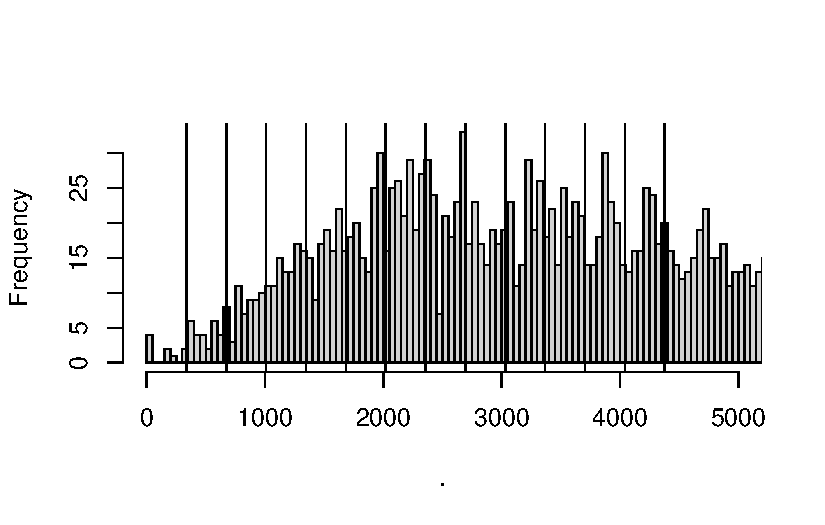
\includegraphics{Tax-Prod_files/figure-pdf/fig-revenue-hist-bunch-0-1.pdf}

}

\end{figure}%

\begin{figure}

\caption{\label{fig-revenue-hist-bunch-1}Revenue distribution Limited
Partnership (81-83)}

\centering{

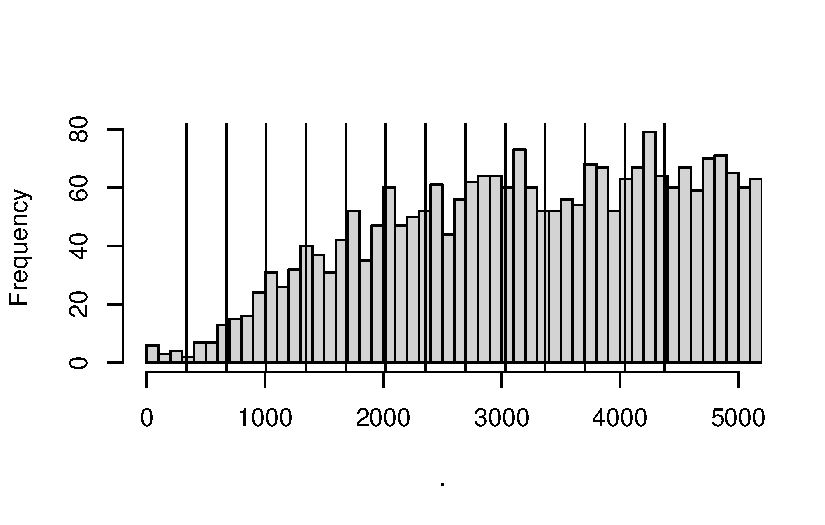
\includegraphics{Tax-Prod_files/figure-pdf/fig-revenue-hist-bunch-1-1.pdf}

}

\end{figure}%

\begin{equation}\phantomsection\label{eq-reg-tax-jo}{
log(s_{it})= \Phi(k_{it},l_{it},m_{it})+ \alpha_1Tax_{it}+\mathbf{\beta}_1'JurOrg_i + \beta_2'JurOrg_i\times\gamma_t+ \gamma_t + \gamma_{ind} +\gamma_{metro} + \varepsilon_{it}
}\end{equation}

\begin{table}

\caption{\label{tbl-reg-jo-tax}Effect of the Juridical Organization Type
and Sales Tax on the Log Share of Intermediate Inputs.}

\begin{minipage}{\linewidth}

\begingroup
\centering
\begin{tabular}{lccc}
   \tabularnewline \midrule \midrule
   Dependent Variable: & \multicolumn{3}{c}{\(log(s)\)}\\
   Model:            & (1)            & (2)             & (3)\\  
   \midrule
   \emph{Variables}\\
   Sales Tax Rate    & 0.2726$^{**}$  & 0.3718$^{***}$  & 0.3481$^{***}$\\   
                     & (0.1210)       & (0.0998)        & (0.0996)\\   
   Proprietorships   & 0.1551$^{***}$ & 0.1243$^{***}$  & 0.1208$^{***}$\\   
                     & (0.0290)       & (0.0219)        & (0.0215)\\   
   Ld. Liability Co. & 0.1707$^{***}$ & 0.1421$^{***}$  & 0.1370$^{***}$\\   
                     & (0.0302)       & (0.0239)        & (0.0240)\\   
   Collective        & 0.2159$^{***}$ & 0.1799$^{***}$  & 0.1829$^{***}$\\   
                     & (0.0556)       & (0.0510)        & (0.0505)\\   
   De Facto Corp.    & 0.1803$^{***}$ & 0.1537$^{***}$  & 0.1512$^{***}$\\   
                     & (0.0316)       & (0.0275)        & (0.0261)\\   
   Joint Partnership & 0.1854$^{***}$ & 0.1583$^{***}$  & 0.1565$^{***}$\\   
                     & (0.0338)       & (0.0275)        & (0.0288)\\   
   Joint Stock Co.   & 0.0696$^{*}$   & 0.0373          & 0.0384\\   
                     & (0.0381)       & (0.0323)        & (0.0330)\\   
   Cooperative       & 0.2585$^{***}$ & 0.2155$^{***}$  & 0.2203$^{***}$\\   
                     & (0.0729)       & (0.0656)        & (0.0648)\\   
   Official Entity   & 0.0612         & 0.1200$^{*}$    & 0.1263$^{*}$\\   
                     & (0.0626)       & (0.0598)        & (0.0582)\\   
   Religious Comm.   & -0.3549$^{**}$ & -0.4020$^{***}$ & -0.4023$^{***}$\\   
                     & (0.1159)       & (0.1260)        & (0.1231)\\   
   \midrule
   \emph{Fixed-effects}\\
   Industry          &                & Yes             & Yes\\  
   Metro Area        &                &                 & Yes\\  
   \midrule
   \emph{Fit statistics}\\
   Observations      & 41,830         & 41,830          & 41,830\\  
   R$^2$             & 0.55169        & 0.56490         & 0.57002\\  
   Within R$^2$      &                & 0.51876         & 0.52096\\  
   \midrule \midrule
   \multicolumn{4}{l}{\emph{Clustered (Industry \& Year) standard-errors in parentheses}}\\
   \multicolumn{4}{l}{\emph{Signif. Codes: ***: 0.01, **: 0.05, *: 0.1}}\\
\end{tabular}

\end{minipage}%
\newline
\begin{minipage}{\linewidth}

\par \raggedright

\end{minipage}%
\newline
\begin{minipage}{\linewidth}

Reference group is Corporations in 1981.

\end{minipage}%
\newline
\begin{minipage}{\linewidth}

\par\endgroup

\end{minipage}%

\end{table}%

\begin{equation}\phantomsection\label{eq-reg-tax-fp}{
log(s_{it})= \Phi(k_{it},l_{it},m_{it})+ \beta_1'JurOrg_i + \beta_2'FiscalPd+\beta_2'JurOrg_i\times FiscalPd + \gamma_t + \gamma_{ind} +\gamma_{metro} + \varepsilon_{it}
}\end{equation}

\begin{table}

\caption{\label{tbl-reg-fiscal-p}Effect of the Type of Juridical
Organization on the Log Share of Intermediate Inputs, per Fiscal
Period.}

\begin{minipage}{\linewidth}

\begingroup
\centering
\begin{tabular}{lccc}
   \tabularnewline \midrule \midrule
   Dependent Variable: & \multicolumn{3}{c}{\(log(s)\)}\\
   Model:                            & (1)             & (2)            & (3)\\  
   \midrule
   \emph{Variables}\\
   Proprietorships                   & 0.1528$^{***}$  & 0.1244$^{***}$ & 0.1207$^{***}$\\   
                                     & (0.0278)        & (0.0210)       & (0.0207)\\   
   Proprietorships $\times$ Year 82  & -0.0116         & -0.0093        & -0.0086\\   
                                     & (0.0129)        & (0.0138)       & (0.0141)\\   
   Proprietorships $\times$ Year 83  & -0.0256$^{*}$   & -0.0233$^{*}$  & -0.0192\\   
                                     & (0.0131)        & (0.0117)       & (0.0118)\\   
   Proprietorships $\times$ Year 84  & -0.0360$^{***}$ & -0.0326$^{**}$ & -0.0280$^{**}$\\   
                                     & (0.0070)        & (0.0112)       & (0.0121)\\   
   Proprietorships $\times$ Year 85  & -0.0441$^{***}$ & -0.0384$^{**}$ & -0.0324$^{**}$\\   
                                     & (0.0123)        & (0.0146)       & (0.0139)\\   
   Proprietorships $\times$ Year 86  & -0.0500$^{***}$ & -0.0428$^{**}$ & -0.0351$^{*}$\\   
                                     & (0.0132)        & (0.0166)       & (0.0182)\\   
   Proprietorships $\times$ Year 87  & -0.0495$^{***}$ & -0.0403$^{**}$ & -0.0343$^{*}$\\   
                                     & (0.0137)        & (0.0153)       & (0.0165)\\   
   Proprietorships $\times$ Year 88  & -0.0615$^{***}$ & -0.0521$^{**}$ & -0.0454$^{**}$\\   
                                     & (0.0153)        & (0.0182)       & (0.0201)\\   
   Proprietorships $\times$ Year 89  & -0.0624$^{**}$  & -0.0528$^{**}$ & -0.0440\\   
                                     & (0.0212)        & (0.0220)       & (0.0244)\\   
   Proprietorships $\times$ Year 90  & -0.0395         & -0.0286        & -0.0192\\   
                                     & (0.0288)        & (0.0296)       & (0.0319)\\   
   Proprietorships $\times$ Year 91  & -0.0375         & -0.0225        & -0.0132\\   
                                     & (0.0400)        & (0.0404)       & (0.0431)\\   
   \midrule
   \emph{Fixed-effects}\\
   Industry                          &                 & Yes            & Yes\\  
   Metro Area                        &                 &                & Yes\\  
   \midrule
   \emph{Fit statistics}\\
   Observations                      & 41,830          & 41,830         & 41,830\\  
   R$^2$                             & 0.55040         & 0.56338        & 0.56869\\  
   Within R$^2$                      &                 & 0.51708        & 0.51948\\  
   \midrule \midrule
   \multicolumn{4}{l}{\emph{Clustered (Industry \& Year) standard-errors in parentheses}}\\
   \multicolumn{4}{l}{\emph{Signif. Codes: ***: 0.01, **: 0.05, *: 0.1}}\\
\end{tabular}

\end{minipage}%
\newline
\begin{minipage}{\linewidth}

\par \raggedright

\end{minipage}%
\newline
\begin{minipage}{\linewidth}

Reference group is Corporations in 1981

\end{minipage}%
\newline
\begin{minipage}{\linewidth}

\par\endgroup

\end{minipage}%

\end{table}%

\begin{table}

\caption{\label{tbl-reg-energy}Effect of the Juridical Organization Type
and Sales Tax on the Log Share of Consumed Energy.}

\begin{minipage}{\linewidth}

\begingroup
\centering
\begin{tabular}{lccc}
   \tabularnewline \midrule \midrule
   Dependent Variable: & \multicolumn{3}{c}{\(log(Energy/Revenue)\)}\\
   Model:            & (1)            & (2)            & (3)\\  
   \midrule
   \emph{Variables}\\
   Sales Tax Rate    & 0.3320$^{**}$  & 0.4223$^{***}$ & 0.3996$^{***}$\\   
                     & (0.1359)       & (0.1075)       & (0.1124)\\   
   Proprietorships   & 0.1420$^{***}$ & 0.1090$^{***}$ & 0.1084$^{***}$\\   
                     & (0.0247)       & (0.0183)       & (0.0182)\\   
   Ld. Liability Co. & 0.1594$^{***}$ & 0.1284$^{***}$ & 0.1252$^{***}$\\   
                     & (0.0262)       & (0.0190)       & (0.0192)\\   
   Collective        & 0.1786$^{***}$ & 0.1389$^{***}$ & 0.1444$^{***}$\\   
                     & (0.0414)       & (0.0353)       & (0.0356)\\   
   De Facto Corp.    & 0.1573$^{***}$ & 0.1301$^{***}$ & 0.1277$^{***}$\\   
                     & (0.0283)       & (0.0257)       & (0.0249)\\   
   Joint Partnership & 0.1719$^{***}$ & 0.1426$^{***}$ & 0.1368$^{***}$\\   
                     & (0.0325)       & (0.0266)       & (0.0271)\\   
   Joint Stock Co.   & 0.0722$^{*}$   & 0.0367         & 0.0326\\   
                     & (0.0391)       & (0.0328)       & (0.0327)\\   
   Cooperative       & 0.2357$^{***}$ & 0.1886$^{**}$  & 0.1916$^{**}$\\   
                     & (0.0689)       & (0.0620)       & (0.0624)\\   
   Official Entity   & -0.0192        & 0.0367         & 0.0422\\   
                     & (0.0587)       & (0.0504)       & (0.0493)\\   
   Religious Comm.   & -0.3095$^{**}$ & -0.3553$^{**}$ & -0.3526$^{**}$\\   
                     & (0.1035)       & (0.1131)       & (0.1124)\\   
   \midrule
   \emph{Fixed-effects}\\
   Industry          &                & Yes            & Yes\\  
   Metro Area        &                &                & Yes\\  
   \midrule
   \emph{Fit statistics}\\
   Observations      & 41,547         & 41,547         & 41,547\\  
   R$^2$             & 0.95296        & 0.95450        & 0.95491\\  
   Within R$^2$      &                & 0.94766        & 0.94566\\  
   \midrule \midrule
   \multicolumn{4}{l}{\emph{Clustered (Industry \& Year) standard-errors in parentheses}}\\
   \multicolumn{4}{l}{\emph{Signif. Codes: ***: 0.01, **: 0.05, *: 0.1}}\\
\end{tabular}

\end{minipage}%
\newline
\begin{minipage}{\linewidth}

\par \raggedright

\end{minipage}%
\newline
\begin{minipage}{\linewidth}

Reference group is Corporations in 1981.

\end{minipage}%
\newline
\begin{minipage}{\linewidth}

\par\endgroup

\end{minipage}%

\end{table}%

\begin{table}

\caption{\label{tbl-reg-ded}Effect of the Juridical Organization Type
and Sales Tax on the Log Share of Deductible Expenses.}

\begin{minipage}{\linewidth}

\begingroup
\centering
\begin{tabular}{lccc}
   \tabularnewline \midrule \midrule
   Dependent Variable: & \multicolumn{3}{c}{Log Share of Deductibles}\\
   Model:            & (1)            & (2)            & (3)\\  
   \midrule
   \emph{Variables}\\
   Sales Tax Rate    & 0.1345         & 0.3305$^{**}$  & 0.3248$^{**}$\\   
                     & (0.1803)       & (0.1123)       & (0.1142)\\   
   Proprietorships   & 0.2203$^{***}$ & 0.1759$^{***}$ & 0.1735$^{***}$\\   
                     & (0.0301)       & (0.0215)       & (0.0216)\\   
   Ld. Liability Co. & 0.2122$^{***}$ & 0.1746$^{***}$ & 0.1736$^{***}$\\   
                     & (0.0319)       & (0.0224)       & (0.0224)\\   
   Collective        & 0.2312$^{***}$ & 0.1883$^{***}$ & 0.1924$^{***}$\\   
                     & (0.0418)       & (0.0334)       & (0.0355)\\   
   De Facto Corp.    & 0.2416$^{***}$ & 0.2005$^{***}$ & 0.1974$^{***}$\\   
                     & (0.0351)       & (0.0300)       & (0.0306)\\   
   Joint Partnership & 0.2224$^{***}$ & 0.1942$^{***}$ & 0.1934$^{***}$\\   
                     & (0.0397)       & (0.0329)       & (0.0337)\\   
   Joint Stock Co.   & 0.0860$^{**}$  & 0.0466         & 0.0419\\   
                     & (0.0363)       & (0.0315)       & (0.0317)\\   
   Cooperative       & 0.2641$^{***}$ & 0.2108$^{**}$  & 0.2064$^{**}$\\   
                     & (0.0820)       & (0.0738)       & (0.0741)\\   
   Official Entity   & 0.0419         & 0.1099$^{*}$   & 0.1087$^{*}$\\   
                     & (0.0604)       & (0.0572)       & (0.0571)\\   
   Religious Comm.   & -0.2153$^{*}$  & -0.2652$^{*}$  & -0.2748$^{*}$\\   
                     & (0.1182)       & (0.1327)       & (0.1375)\\   
   \midrule
   \emph{Fixed-effects}\\
   Industry          &                & Yes            & Yes\\  
   Metro Area        &                &                & Yes\\  
   \midrule
   \emph{Fit statistics}\\
   Observations      & 41,824         & 41,824         & 41,824\\  
   R$^2$             & 0.74688        & 0.75949        & 0.76154\\  
   Within R$^2$      &                & 0.73059        & 0.73187\\  
   \midrule \midrule
   \multicolumn{4}{l}{\emph{Clustered (Industry \& Year) standard-errors in parentheses}}\\
   \multicolumn{4}{l}{\emph{Signif. Codes: ***: 0.01, **: 0.05, *: 0.1}}\\
\end{tabular}

\end{minipage}%
\newline
\begin{minipage}{\linewidth}

\par \raggedright

\end{minipage}%
\newline
\begin{minipage}{\linewidth}

Reference group is Corporations in 1981.

\end{minipage}%
\newline
\begin{minipage}{\linewidth}

\par\endgroup

\end{minipage}%

\end{table}%

\begin{table}

\caption{\label{tbl-reg-non-ded}Effect of the Juridical Organization
Type and Sales Tax on the Log Share of Non-Deductible Expenses.}

\begin{minipage}{\linewidth}

\begingroup
\centering
\begin{tabular}{lccc}
   \tabularnewline \midrule \midrule
   Dependent Variable: & \multicolumn{3}{c}{log(non\_deductibles/sales)}\\
   Model:            & (1)            & (2)            & (3)\\  
   \midrule
   \emph{Variables}\\
   Sales Tax Rate    & 0.1345         & 0.3305$^{**}$  & 0.3248$^{**}$\\   
                     & (0.1803)       & (0.1123)       & (0.1142)\\   
   Proprietorships   & 0.2203$^{***}$ & 0.1759$^{***}$ & 0.1735$^{***}$\\   
                     & (0.0301)       & (0.0215)       & (0.0216)\\   
   Ld. Liability Co. & 0.2122$^{***}$ & 0.1746$^{***}$ & 0.1736$^{***}$\\   
                     & (0.0319)       & (0.0224)       & (0.0224)\\   
   Collective        & 0.2312$^{***}$ & 0.1883$^{***}$ & 0.1924$^{***}$\\   
                     & (0.0418)       & (0.0334)       & (0.0355)\\   
   De Facto Corp.    & 0.2416$^{***}$ & 0.2005$^{***}$ & 0.1974$^{***}$\\   
                     & (0.0351)       & (0.0300)       & (0.0306)\\   
   Joint Partnership & 0.2224$^{***}$ & 0.1942$^{***}$ & 0.1934$^{***}$\\   
                     & (0.0397)       & (0.0329)       & (0.0337)\\   
   Joint Stock Co.   & 0.0860$^{**}$  & 0.0466         & 0.0419\\   
                     & (0.0363)       & (0.0315)       & (0.0317)\\   
   Cooperative       & 0.2641$^{***}$ & 0.2108$^{**}$  & 0.2064$^{**}$\\   
                     & (0.0820)       & (0.0738)       & (0.0741)\\   
   Official Entity   & 0.0419         & 0.1099$^{*}$   & 0.1087$^{*}$\\   
                     & (0.0604)       & (0.0572)       & (0.0571)\\   
   Religious Comm.   & -0.2153$^{*}$  & -0.2652$^{*}$  & -0.2748$^{*}$\\   
                     & (0.1182)       & (0.1327)       & (0.1375)\\   
   \midrule
   \emph{Fixed-effects}\\
   Industry          &                & Yes            & Yes\\  
   Metro Area        &                &                & Yes\\  
   \midrule
   \emph{Fit statistics}\\
   Observations      & 41,824         & 41,824         & 41,824\\  
   R$^2$             & 0.94466        & 0.94742        & 0.94787\\  
   Within R$^2$      &                & 0.93972        & 0.93789\\  
   \midrule \midrule
   \multicolumn{4}{l}{\emph{Clustered (Industry \& Year) standard-errors in parentheses}}\\
   \multicolumn{4}{l}{\emph{Signif. Codes: ***: 0.01, **: 0.05, *: 0.1}}\\
\end{tabular}

\end{minipage}%
\newline
\begin{minipage}{\linewidth}

\par \raggedright

\end{minipage}%
\newline
\begin{minipage}{\linewidth}

Reference group is Corporations in 1981.

\end{minipage}%
\newline
\begin{minipage}{\linewidth}

\par\endgroup

\end{minipage}%

\end{table}%

\subsection{Do Corporations in Colombia have different technologies than
other juridical
organizations?}\label{do-corporations-in-colombia-have-different-technologies-than-other-juridical-organizations}

An implicit assumption in the identification strategy is that the subset
of non-evaders has the same common technology as evaders. In the case of
Colombia, this implies that Corporations have the same common technology
as Proprietorships, Limited Companies, and Partnerships. However, we can
think that firms with better technology are self-selecting into
corporations, and thus, firms with low-performance technology will be
mislabeled as evaders.

The key question is how firms are choosing their juridical organization,
and in particular, how firms are choosing to become corporations. I
argue that choosing the juridical organization is a result of the
capital needs of the firm and it is affected by the preferences of the
owners over their corporate liability and their social connections.

From the definitions of the juridical organizations, we can expect
corporations to be the largests in terms of capital, followed by LLCs
and Partnerships, and Proprietorships to be smallest. The reason is
simply that more people can participate by contributing their capital to
the firm. This ordering in turn would suggest a growth path for the
firms.

Turning to the data, I find some firms change their juridical
organization type. I build a juridical organization transition matrix
from the previous year to the next one at the firm level.
Table~\ref{tbl-trans-mat} shows the transition matrix. Although the
transition matrix suggests that firms mostly stay in their juridical
organization, a growth trend emerges. It looks like proprietorships turn
into LLCs, and LLCs into Corporations.

\begin{table}

\caption{\label{tbl-trans-mat}Transition Matrix}

\centering{

\centering
\begin{tabular}[t]{l|r|r|r|r|r}
\hline
  & Corporation & Ltd. Co. & Other & Partnership & Proprietorship\\
\hline
Corporation & 7758 & 36 & 1 & 10 & 0\\
\hline
Ltd. Co. & 228 & 21843 & 5 & 32 & 46\\
\hline
Other & 1 & 5 & 446 & 0 & 1\\
\hline
Partnership & 16 & 69 & 0 & 1150 & 6\\
\hline
Proprietorship & 4 & 196 & 0 & 31 & 4173\\
\hline
\end{tabular}

}

\end{table}%

Looking into the capital distributions of proprietorships, LLCs, and
corporations we find that corporations are the largest, followed by
LLCs, and proprietorships are the smallest
Figure~\ref{fig-k-rev-hist-1}. However, there are considerable overlaps.
The same is true for revenues (in logs) Figure~\ref{fig-k-rev-hist-2}.
This is not surprising, as the need for larger capital increases, the
more people would need to participate.

However, when we look at the frequency distributions of the capital over
revenue ratio in logs, the distributions perfectly overlap
Figure~\ref{fig-k-rev-hist-3}. If corporations had different
technologies we would expect to see two different distributions. In
particular, the distribution of corporations would have been farther to
the right than the distributions of proprietorships and LLCs.

These patterns remain even after controlling for industry, metropolitan
area, and year Table~\ref{tbl-reg-choosing-jo}.

\begin{figure}

\begin{minipage}{0.50\linewidth}

\centering{

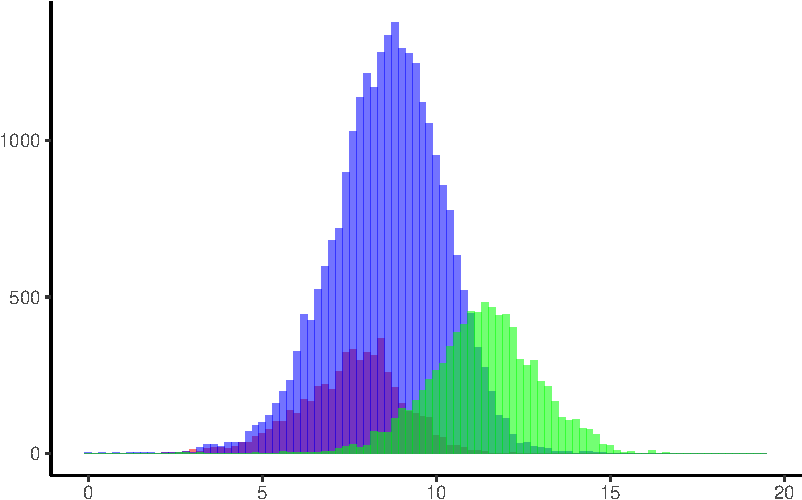
\includegraphics{Tax-Prod_files/figure-pdf/fig-k-rev-hist-1.pdf}

}

\subcaption{\label{fig-k-rev-hist-1}Capital}

\end{minipage}%
%
\begin{minipage}{0.50\linewidth}

\centering{

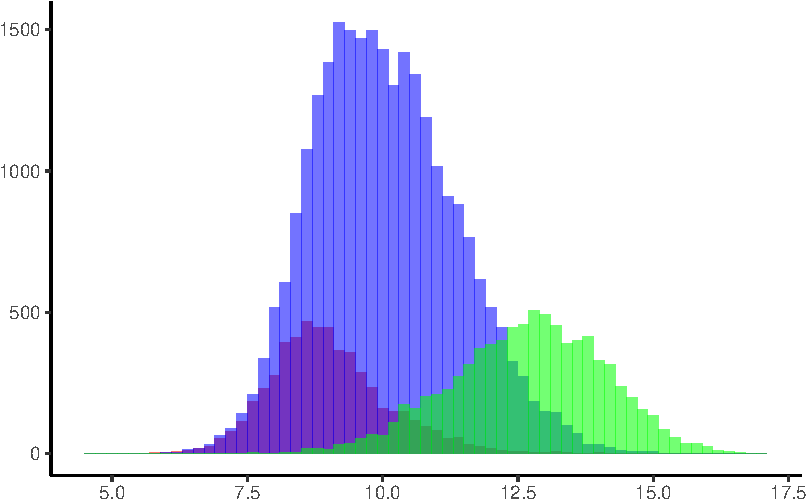
\includegraphics{Tax-Prod_files/figure-pdf/fig-k-rev-hist-2.pdf}

}

\subcaption{\label{fig-k-rev-hist-2}Revenue}

\end{minipage}%
\newline
\begin{minipage}{\linewidth}

\centering{

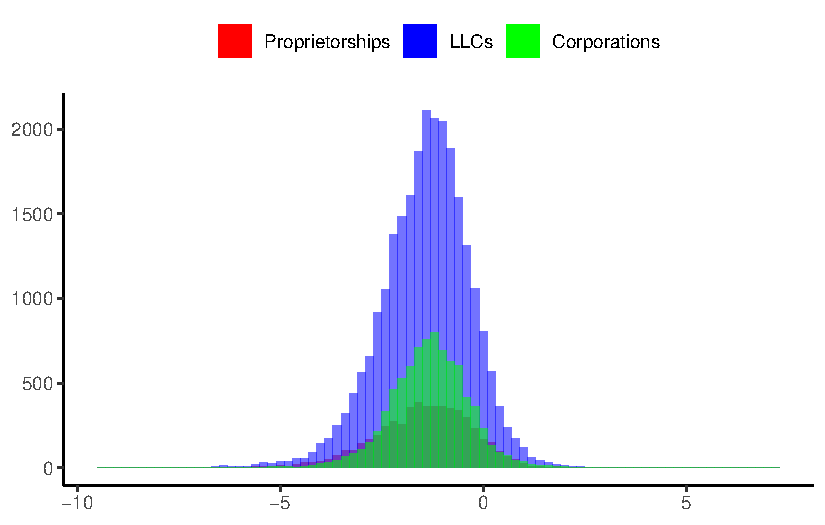
\includegraphics{Tax-Prod_files/figure-pdf/fig-k-rev-hist-3.pdf}

}

\subcaption{\label{fig-k-rev-hist-3}Capital/Revenue}

\end{minipage}%

\caption{\label{fig-k-rev-hist}Frequency historgrams of capital, revenue
and capital/revenue (in logs) of Corporations, LLCs, and
Proprietorships.}

\end{figure}%

\begin{table}

\caption{\label{tbl-reg-choosing-jo}Testing Differences in the log of
Capital, Revenue, and Capital/Revenue for Corporations and Other
Juridical Organizations}

\begin{minipage}{\linewidth}

\begingroup
\centering
\begin{tabular}{lccc}
   \tabularnewline \midrule \midrule
   Dependent Variables:                    & log(capital)   & log(sales)     & log(capital/sales)\\  
   Model:                                  & (1)            & (2)            & (3)\\  
   \midrule
   \emph{Variables}\\
   juridical\_organizationLLCs             & -2.446$^{***}$ & -2.424$^{***}$ & -0.0212\\   
                                           & (0.0743)       & (0.0639)       & (0.0601)\\   
   juridical\_organizationProprietorships  & -3.346$^{***}$ & -3.372$^{***}$ & 0.0265\\   
                                           & (0.1672)       & (0.1220)       & (0.0897)\\   
   \midrule
   \emph{Fixed-effects}\\
   Industry                                & Yes            & Yes            & Yes\\  
   Metro Area                              & Yes            & Yes            & Yes\\  
   Year                                    & Yes            & Yes            & Yes\\  
   \midrule
   \emph{Fit statistics}\\
   Observations                            & 39,628         & 39,628         & 39,628\\  
   R$^2$                                   & 0.44574        & 0.51147        & 0.12003\\  
   Within R$^2$                            & 0.31430        & 0.39972        & 0.00025\\  
   \midrule \midrule
   \multicolumn{4}{l}{\emph{Clustered (Industry \& Year) standard-errors in parentheses}}\\
   \multicolumn{4}{l}{\emph{Signif. Codes: ***: 0.01, **: 0.05, *: 0.1}}\\
\end{tabular}
\par\endgroup

\end{minipage}%

\end{table}%

\subsubsection{Model of firm (capital) growth
(sketch)}\label{model-of-firm-capital-growth-sketch}

A limited liability company looking to acquire more capital had three
options.

First, partners can increase their capital participation, using personal
wealth or through a bank credit. This option however will increase the
partners' liability. The more capital I bring the greater my liability
is.

Second, the LLC might increase its capital by inviting additional
partners. As the firm increases its capital, inviting more partners will
become more difficult. The funding partners risk losing control of their
firm, as more people participate in the firm's management and
decision-making.

Third, the firm can incorporate. This will bring capital to the firm.
Anyone in the market for the shares of the firm can participate. Shares
can be traded. A CEO reporting to the shareholders might be appointed.
Liability is limited to shares.

The decision to incorporate is a decision on how to acquire capital.
Firms still need to consider the stream of future productivity shocks,
but the decision also depends on other unobservables such as
risk-aversion (increasing the partners' liability), the partners'
ability to convince more partners to join the LLC, and preferences over
the control of the firm's management.

Assume there's an unobserved scalar \(\zeta_i\) that captures all of the
owners' heterogeneity in preferences over liability risk, access to
networks of potential investors, and preferences over the control of the
firm's management. Let a higher value of \(\zeta\) capture less risk
aversion, a wider network of potential investors, or a higher preference
for retaining control over the firm. Consider the case in which two LLCs
firms are looking to optimally increase their capital by the same
quantity, but the owners are different in \(\zeta\). In particular, let
the owner of firm 1 have a higher \(\zeta_1>\zeta_2\) than the owner of
firm 2. The firms also have the same technology and productivity shocks.
The owner of firm 1 \(\zeta_1\) would be able to convince additional
investors to join their LLC, but the owner 2 \(\zeta_2\) would not.
\(\zeta_2\) owner would have to choose to incorporate to get the capital
for his firm or forgo growth.

The 20 pp difference in CIT rate between LLCs and Corporations might
have deterred firm growth. The CIT was homogenized to 30\% in 1986. What
was the capital misallocation due to the tax rate differential? Are more
firms incorporating after the reform?

\subsubsection{Evasion vs.~Production
Technology}\label{evasion-vs.-production-technology}

Production technology is industry-specific, but evasion technology is
the same across industries.

Take the face value of the regressions and assume, without conceding,
that corporations have different technologies. This will imply that
corporations have technologies that are consistently 15\% more
productive than non-corporations regardless of the industry. In other
words, it does not matter if the firms produce canned food, shoes or
furniture, corporations have technologies consistently more productive.
However, this is difficult to believe because there could be industries
in which such an improvement in technology is difficult to imagine. For
example, coffee grain mills (food products), steel foundries (steel
basic products), plastic molding and extrusion (plastic products), or
cement (non-metallic mineral products).

However, these cross-sectional differences across industries could be
better explained by the evasion technology. We would expect the evasion
technology to be the same across industries. It does not matter what I
produce and what technology my firm employs, to overreport inputs all
that is needed is a fake invoice.

\subsubsection{Corporations by Industry}\label{corporations-by-industry}

Looking into industry sectors.

\begin{table}

\caption{\label{tbl-corps-by-inds}Corporations by Industry. Top 20
Industries in Colombia by number of firms.}

\centering{

\centering
\begin{tabular}[t]{r|r|r|r|r|r|l}
\hline
sic\_3 & n\_sic & corps\_n & corps\_share & market\_share & n\_perc & Descripción\\
\hline
313 & 1419 & 837 & 58.99 & 7.43 & 1.87 & Beverage industries\\
\hline
351 & 1360 & 740 & 54.41 & 6.97 & 1.79 & Manufacture of industrial chemicals\\
\hline
352 & 3274 & 1001 & 30.57 & 6.55 & 4.32 & Manufacture of other chemical products\\
\hline
341 & 1560 & 409 & 26.22 & 4.07 & 2.06 & Manufacture of paper and paper products\\
\hline
383 & 2174 & 532 & 24.47 & 3.03 & 2.87 & Manufacture of electrical machinery apparatus, appliances and supplies\\
\hline
369 & 3333 & 663 & 19.89 & 3.41 & 4.40 & Manufacture ot other non-metallic mineral products\\
\hline
312 & 2201 & 422 & 19.17 & 4.80 & 2.90 & Food manufacturing\\
\hline
384 & 2491 & 385 & 15.46 & 5.21 & 3.29 & Manufacture of transport equipment\\
\hline
321 & 5158 & 771 & 14.95 & 7.56 & 6.80 & Manufacture of textiles\\
\hline
311 & 11049 & 1613 & 14.60 & 20.40 & 14.57 & Food manufacturing\\
\hline
356 & 3400 & 491 & 14.44 & 2.96 & 4.48 & Manufacture of plastic products not elsewhere classified\\
\hline
381 & 6231 & 761 & 12.21 & 3.26 & 8.22 & Manufacture of fabricated metal products, except machinery and equipment\\
\hline
323 & 1086 & 129 & 11.88 & 0.97 & 1.43 & Manufacture of leather and products of leather, leather substitutes and fur, except footwear and wearing apparel\\
\hline
331 & 1971 & 220 & 11.16 & 0.61 & 2.60 & Manufacture of wood and wood and cork products, except furniture\\
\hline
382 & 3474 & 339 & 9.76 & 1.66 & 4.58 & Manufacture of machinery except electrical\\
\hline
342 & 3943 & 376 & 9.54 & 2.54 & 5.20 & Printing, publishing and allied industries\\
\hline
390 & 1726 & 130 & 7.53 & 0.81 & 2.28 & Other manufacturing industries\\
\hline
332 & 2225 & 73 & 3.28 & 0.37 & 2.93 & Manufacture of furniture and fixtures, except primarily of metal\\
\hline
324 & 2833 & 91 & 3.21 & 0.99 & 3.74 & Manufacture of footwear, except vulcanized ord moulded rubber or plastic footwear\\
\hline
322 & 10819 & 254 & 2.35 & 2.79 & 14.27 & Manufacture of wearing apparel, except footwear\\
\hline
\end{tabular}

}

\end{table}%

\subsubsection{Inputs Cost Share of
Revenues}\label{inputs-cost-share-of-revenues}

The evidence suggests that Corporations have similar technologies to the
rest of the firms. I look at the share of revenues of different input
costs. In doing so, I consider the incentives generated by the fiscal
environment in Colombia. Firms had the lowest incentives to evade taxes
by misreporting capital, consumed energy, and skilled labor. The cost
share of revenue of these inputs suggests that Corporations and the rest
of the firms had the same technologies.

\paragraph{Capital}\label{capital}

Firms could not deduct capital goods from sales taxes. However, firms of
capital-intensive industries might have had incentives to underreport
capital because capital was used to set the minimum income tax. Income
tax could not be less than 8 percent of the capital.

\paragraph{Energy}\label{energy}

Before the electrical energy reform in 1994, the power market was almost
exclusively supplied by public companies with negligible participation
from private firms. The public companies were inefficient and suffered
financial distress due to poor management and low tariffs set by
political actors. Two major blackouts in 1983 and 1992-1993 led to the
1994 reform that opened the sector to private participation.

It is unlikely that firms overreported energy, as they have to purchase
from a Corporation or a public company. Both of those organizations had
no incentives to cooperate and provide fake invoices.

In the data, energy sold by corporations accounted on average for 73\%
of the total energy sold, but only 1.7\% of the total energy purchased.
In addition, corporations sold energy at 12 times the market price on
average Table~\ref{tbl-energy}. The high price might suggest
corporations had market power in the electric energy market, however,
this is unlikely to be relevant to affect any estimations as their
overall market share is small.

\begin{table}

\caption{\label{tbl-energy}Electric energy market in Colombia
(1981-1991).}

\centering{

\centering
\begin{tabular}[t]{l|r|r|r|r}
\hline
 & Sold/Purchased Price Ratio & Sold Energy (\% of Total Sold Energy) & Sold Energy (\% of Total Purchased Energy) & Generated Energy (\% of Consumed Energy)\\
\hline
Corporation & 11.9 & 73.0 & 1.7 & 3.7\\
\cline{1-5}
Ltd. Co. & 7.4 & 2.1 & 0.0 & 0.2\\
\cline{1-5}
Other & 2.5 & 24.8 & 0.6 & 5.3\\
\cline{1-5}
Partnership & 1.0 & 0.0 & 0.0 & 0.7\\
\cline{1-5}
Proprietorship & 1.0 & 0.0 & 0.0 & 0.1\\
\hline
\end{tabular}

}

\end{table}%

\paragraph{Labor}\label{labor}

Firms might have incentives to underreport labor to evade Payroll Taxes
(PRT) if the expected benefits of evading the PRT outweigh the
opportunity costs of evading Corporate Income Tax (CIT) by overreporting
labor costs and the expected cost of evading PRT \citep{Almunia2018}.

Firms are more likely to underreport unskilled rather than skilled
labor. Skilled employees are less likely to cooperate with firms in
underreporting their wages. Firms might offer employees cash
compensations in order for employees to accept lower reported wages or
report their wages at all. The cost for employees is that these payroll
taxes provide them with social benefits such as social security or
public health access. These benefits are not obvious in the short run.
It is more likely that unskilled labor to be short-sighted and accept to
cooperate with firms to underreport their wages. Skilled workers, on the
other hand, are less likely to accept these conditions and to have
outside options and move if the conditions are not favorable to them.

\paragraph{Services and other
expenditures}\label{services-and-other-expenditures}

The Colombian dataset allows, to some extent, separating expenditures,
including services, into deductible and non-deductible expenses. In
contrast to non-evading firms, evading firms should use a higher share
of deductible expenses. The reason is that firms have incentives to
overreport deductible expenditure to evade ICT and VAT.

The Colombian data separates firms' total expenditures into general and
industrial expenditures. Industrial expenditure is defined as the
indirect costs and expenditures incurred by the firm in order to perform
its industrial activity. The data lists the purchase of accessories and
replacement parts, fuels and lubricants consumed by the establishment,
industrial work by other establishments, and third-party repairs and
maintenance, among others, as industrial expenditures\footnote{After
  1992, industrial expenditure included rent of machinery and property,
  payment for professional services, insurance (excluding employee
  benefits), water, mail, and telephone.}. All other expenses, including
insurance (excluding employee benefits) and machinery rentals, are
considered general expenses.

Most services were excluded from sales taxes. Some non-excluded services
in this period were insurance premiums (excluding life insurance),
repair and maintenance, national and international telegrams, telex, and
telephone, and rental of goods and chattels, including financial
leasing.

I classify as deductible expenses the following industrial expenditures:
purchase of fuels and lubricants, payments to third parties for repair
and maintenance, purchase of raw materials and goods sold without
transformation; and the following general expenditures: machinery
rental, insurance excluding employee benefits, and water, mail and
telephone expenses.

\paragraph{Technical note}\label{technical-note}

According to the notes on the dataset, the quantity of energy consumed
by firms is estimated as the difference between purchased plus generated
energy and sold energy. In contrast, the value of consumed energy is the
difference between the value of purchased and sold energy. Consequently,
using the calculated value over the calculated quantity of consumed
energy ignores the quantity of generated energy and the increase in the
price of sold energy by corporations.

In \citet{Gandhi2020}, services are defined as general expenditures
minus machinery rental and interest payments. However, this approach
does not include industrial expenditures which are closely linked to the
production process. In the Colombian data, the intermediate consumption
is defined as raw materials, purchased electric energy, and industrial
expenditure. This definition is close to what is commonly defined as
intermediate inputs.

\paragraph{Results}\label{results}

Table~\ref{tbl-reg-shares} shows that in terms of the capital and
consumed energy share of revenue, corporations are not different from
other types of juridical organizations. Capital and consumed energy are
reliable indicators that Corporations have similar technologies to other
firms because firms have no incentives to overreport capital or consumed
energy. On the other hand, the raw materials share of revenues is 3
percent higher for non-corporations. Firms have incentives to overreport
raw materials to evade sales taxes and CIT. Hence, materials are not a
good reference to compare technology between Corporations and other
types of firms.

Table~\ref{tbl-reg-shares-2} shows that the skilled labor share of
revenue for corporations is not statistically different from other types
of firms. On the other hand, unskilled labor is significantly lower for
non-corporations. Unskilled workers are more likely to cooperate with
non-corporations to underreport their employment/wages. An alternative
explanation is that corporations employ more unskilled workers because
they are bigger. Therefore, skilled labor is a more reliable indicator
of technology and shows that corporations have similar technology to
other firms.

Table~\ref{tbl-reg-shares-2} also shows that the total expenditure share
of revenue is 8 percent lower for non-corporations on average. On one
hand, this might be due to size. Corporations tend to be larger than
non-corporations. However, the composition of the expenditure matters.

Table~\ref{tbl-reg-shares-3} shows that the deductible expenses share of
total expenditure is 6 percent significantly higher for
non-corporations. This is not the case if we classify expenditures by
industrial and general expenses. Services as defined in GNR, that is
general expenses minus machinery rental and interest payments, as a
share of total expenditure is 5 percent higher for non-corporations.
Services include deductible expenses such as insurance excluding
employee benefits, and telegrams and telephone services.

In summary, looking at the inputs that firms are less likely to
misreport due to tax evasion incentives, the evidence suggests that
Corporations have similar technologies to the other types of firms. In
addition, I find that the cost share of inputs that are likely to be
misreported due to tax evasion incentives are significantly different
from corporations and in the expected direction. In particular, it looks
like firms overreport materials and deductible expenses, and underreport
unskilled labor.

\begin{table}

\caption{\label{tbl-reg-shares}Shares of Revenue for different inputs by
Corporations and Non-Corporation.}

\begin{minipage}{\linewidth}

\begingroup
\centering
\begin{tabular}{lccc}
   \tabularnewline \midrule \midrule
   Dependent Variables: & Capital               & Energy                & Materials\\  
   Model:               & (1)                   & (2)                   & (3)\\  
   \midrule
   \emph{Variables}\\
   Non-Corporation      & 0.1524                & -0.1215               & 0.0252$^{**}$\\   
                        & (0.1063)              & (0.7405)              & (0.0092)\\   
   \midrule
   \emph{Fixed-effects}\\
   Industry             & Yes                   & Yes                   & Yes\\  
   Metro Area           & Yes                   & Yes                   & Yes\\  
   Year                 & Yes                   & Yes                   & Yes\\  
   \midrule
   \emph{Fit statistics}\\
   Observations         & 42,145                & 42,145                & 42,145\\  
   R$^2$                & 0.00180               & 0.09753               & 0.01744\\  
   Within R$^2$         & $5.74\times 10^{-5}$  & $1.97\times 10^{-5}$  & 0.00021\\  
   \midrule \midrule
   \multicolumn{4}{l}{\emph{Clustered (Industry \& Year) standard-errors in parentheses}}\\
   \multicolumn{4}{l}{\emph{Signif. Codes: ***: 0.01, **: 0.05, *: 0.1}}\\
\end{tabular}
\par\endgroup

\end{minipage}%

\end{table}%

\begin{table}

\caption{\label{tbl-reg-shares-2}Shares of Revenue for different inputs
by Corporations and Non-Corporation.}

\begin{minipage}{\linewidth}

\begingroup
\centering
\begin{tabular}{lccc}
   \tabularnewline \midrule \midrule
   Dependent Variables: & Skilled Labor         & Unskilled Labor & Total Expenditure\\  
   Model:               & (1)                   & (2)             & (3)\\  
   \midrule
   \emph{Variables}\\
   Non-Corporation      & 0.2052                & 0.0740$^{***}$  & -0.0728$^{***}$\\   
                        & (0.2082)              & (0.0090)        & (0.0076)\\   
   \midrule
   \emph{Fixed-effects}\\
   Industry             & Yes                   & Yes             & Yes\\  
   Metro Area           & Yes                   & Yes             & Yes\\  
   Year                 & Yes                   & Yes             & Yes\\  
   \midrule
   \emph{Fit statistics}\\
   Observations         & 42,145                & 42,145          & 42,145\\  
   R$^2$                & 0.00186               & 0.02102         & 0.01575\\  
   Within R$^2$         & $1.91\times 10^{-5}$  & 0.00288         & 0.00416\\  
   \midrule \midrule
   \multicolumn{4}{l}{\emph{Clustered (Industry \& Year) standard-errors in parentheses}}\\
   \multicolumn{4}{l}{\emph{Signif. Codes: ***: 0.01, **: 0.05, *: 0.1}}\\
\end{tabular}
\par\endgroup

\end{minipage}%

\end{table}%

\begin{table}

\caption{\label{tbl-reg-shares-3}Shares of Total Expenses for different
classifications of expenses by Corporations and Non-Corporation.}

\begin{minipage}{\linewidth}

\begingroup
\centering
\begin{tabular}{lccc}
   \tabularnewline \midrule \midrule
   Dependent Variables: & Services       & Industrial Expenditure & Deductible Expenditure\\  
   Model:               & (1)            & (2)                    & (3)\\  
   \midrule
   \emph{Variables}\\
   Non-Corporation      & 0.0497$^{***}$ & -0.0012                & 0.0475$^{***}$\\   
                        & (0.0079)       & (0.0095)               & (0.0087)\\   
   \midrule
   \emph{Fixed-effects}\\
   Industry             & Yes            & Yes                    & Yes\\  
   Metro Area           & Yes            & Yes                    & Yes\\  
   Year                 & Yes            & Yes                    & Yes\\  
   \midrule
   \emph{Fit statistics}\\
   Observations         & 42,140         & 42,140                 & 42,140\\  
   R$^2$                & 0.12339        & 0.13079                & 0.11923\\  
   Within R$^2$         & 0.00825        & $5.6\times 10^{-6}$    & 0.01176\\  
   \midrule \midrule
   \multicolumn{4}{l}{\emph{Clustered (Industry \& Year) standard-errors in parentheses}}\\
   \multicolumn{4}{l}{\emph{Signif. Codes: ***: 0.01, **: 0.05, *: 0.1}}\\
\end{tabular}
\par\endgroup

\end{minipage}%

\end{table}%

\section{Identification Strategy}\label{identification-strategy}

Because the firms' optimization decisions depend on the fiscal
environment, the identification strategy should be motivated by the
fiscal environment \(\Gamma\). In particular, the identification
strategy will be as good as how well we can tell apart a subset of firms
that have the highest incentive to not evade. For example, in the case
of Spain, the firms above the revenue LTU threshold. In the case of
Colombia, the corporations.

\phantomsection\label{ass-non-ev}
\begin{fbx}{Assumption}{Assumption 3.1: }{Non-Evaders}
\phantomsection\label{ass-non-ev}
Based on the fiscal environment \(\Gamma\), the researcher can identify
a subset of firms \(\theta_i\in\Theta^{NE}\subset \Theta\) that does not
evade taxes by overreporting inputs.

\end{fbx}

For those firms, then \(\mathbb{E}[e_{it}|\theta_i\in\Theta^{NE}]=0\)

In addition, I impose the following timing assumption.

\phantomsection\label{ass-ind}
\begin{fbx}{Assumption}{Assumption 3.2: }{Independence}
\phantomsection\label{ass-ind}
Firms choose overreporting \(e_{it}\) \emph{before }the output shock
\(\varepsilon_{it}\)

\end{fbx}

Assumption \hyperref[ass-ind]{3.2} implies that input overreporting is
independent of the current period output shock,
\(e_{it} \perp \varepsilon_{it}\). In the literature is not rare to
assume that the output shock is not part of the information set of the
firms, \(\varepsilon_{it}\not\in \mathcal{I}_t\) \citep{Gandhi2020}.
Timing and information set assumptions are not uncommon for
identification strategies in production functions and demand estimation
\citep{Ackerberg2021, Ackerberg2019}.

\subsection{Identifying the production function
parameters}\label{identifying-the-production-function-parameters}

The econometrician observes then the overreported inputs in the data,
\(M_{it}=M^*_{it}\exp(e_{it})\)\footnote{Note we can always rewrite
  \(M^*+e=M^*\exp\{a\}\), then \(\exp\{a\}=\frac{e}{M^*}+1\).}. Assume
the production function is Cobb-Douglas,
\(G(M^*_{it}, K_{it}, L_{it})\exp(\omega_{it}+\varepsilon_{it})=M^{*\beta}_{it}K_{it}^{\alpha_K}L_{it}^{\alpha_L}\exp(\omega_{it}+\varepsilon_{it})\).
Then, for the case of Colombia, Equation~\ref{eq-foc:ind} applies since
the type of firms is the juridical organization and the non-evaders are
Corporations. By multiplying both sides by the intermediate inputs and
dividing by the output, we get

\begin{equation}\phantomsection\label{eq-foc-cd}{
\begin{aligned}
    \ln\left(\frac{\rho_t M^*_{it}}{P_{t}Y_{it}}\right)+e_{it}&=\ln\beta + \ln \mathcal{E}- \varepsilon_{it} \\
    &\equiv \ln D^{\mathcal{E}}- \varepsilon_{it} 
\end{aligned}
}\end{equation}

where,
\(\mathcal{E}\equiv \mathbb{E}[\exp(\varepsilon_{it})|\mathcal{I}_{it}]=\mathbb{E}[\exp(\varepsilon_{it})]\).

We can use Equation~\ref{eq-foc-cd} and assumption
\hyperref[ass-non-ev]{3.1} to recover the production function parameter
\(\beta\)

\begin{equation}\phantomsection\label{eq-foc-cd-exp}{
    \mathbb{E}\left[\ln\left(\frac{\rho_t M^*_{it}}{P_{t}Y_{it}}\right)\Bigg| \Theta^{NE}\right]=\ln D^{\mathcal{E}}
}\end{equation}

The constant \(\mathcal{E}\) is also identified \citep{Gandhi2020},

\begin{equation}\phantomsection\label{eq-id-E}{
\mathcal{E}=\mathbb{E}\left[\exp\left(\ln D^{\mathcal{E}}- \ln\left(\frac{\rho_t M^*_{it}}{P_{t}Y_{it}}\right)\right)|\theta^{NE}\right]=\mathbb{E}\left[\exp(\varepsilon_{it})|\theta^{NE}\right]=\mathbb{E}[\exp(\varepsilon_{it})]
}\end{equation}

and, thus, the output elasticity of input, \(\beta\), is also
identified,

\begin{equation}\phantomsection\label{eq-id-beta}{
\beta=\exp\left(\ln D^{\mathcal{E}}-\ln\mathcal{E}\right).
}\end{equation}

\subsection{Identifying Tax Evasion}\label{identifying-tax-evasion}

Having recovered both the flexible input elasticity, \(\beta\), and the
constant \(\mathcal{E}\), for all firms, I can form the following
variable using observed data.

\begin{equation}\phantomsection\label{eq-ob-ev}{
\begin{aligned}
    \mathcal V_{it}\equiv&\ln\left(\frac{\rho_t M_{it}}{P_{t}Y_{it}}\right)-\ln\beta -\ln\mathcal{E}\notag \\
    &=\ln\left(\frac{\rho_tM^*_{it}}{P_{t}Y_{it}}\right)-\ln\beta-\ln\mathcal{E}+e_{it} \notag \\
    &=-\varepsilon_{it} +e_{it}
\end{aligned}
}\end{equation}

By assumption \hyperref[ass-ind]{3.2}, the tax evasion,
\(\varepsilon_{it}\) ,is independent of \(e_{it}\). Note that, from
Equation~\ref{eq-foc-cd}, we also recovered
\(f_{\varepsilon}(\varepsilon)\) the distribution of \(\varepsilon\).
Tax evasion therefore can be recovered up to an independent random
variable by using deconvolution methods.

In particular, from probability theory,

\begin{definition}[]\protect\hypertarget{def-conv}{}\label{def-conv}

\begin{fbx}{Definition}{Definition: }{Convolution}
\phantomsection\label{}
The density of the sum of two \textbf{independent} random variables is
equal to the \textbf{convolution} of the densities of both addends;
hence

\[
h = f*m = \int f(\mathcal Z - \varepsilon)m(\varepsilon)d\varepsilon
\]

where \(f\) is the density of \(\mathcal Z\) (Meister, 2009)

\end{fbx}

\end{definition}

\subsection{Identifying Productivity}\label{identifying-productivity}

Here I show how to recover the rest of the parameters of the production
function, including productivity, and the Markov process of
productivity. We can do it in several ways, depending on our object of
interest.

In the literature, it is not uncommon to assume that productivity
follows a Markov process. That is,

\begin{equation}\phantomsection\label{eq-prod-markov}{
    \omega_{it}=h(\omega_{it-1})+\eta_{it}
}\end{equation}

We can form the following observed variable for a guess of
\(\alpha=(\alpha_K,\alpha_L)\),

\[
\begin{aligned}
    \mathcal W_{it}(\alpha) & \equiv \ln Y_{it} - \beta M_{it}-\alpha_K \ln K_{it}-\alpha_L \ln L_{it}+\beta\mathcal{V}_{it}\\
    & = \omega_{it}(\alpha)+(1-\beta)\varepsilon_{it}
\end{aligned}
\]

If we are interested only in productivity, we could use deconvolution to
learn \(\alpha\) and the distribution of productivity.

Alternatively, if we are interested in also identifying the Markov
process of productivity, we can use the orthogonality we get from
Equation~\ref{eq-prod-markov},
\(\mathbb{E}[\eta_{it}|k_{it},l_{it},k_{it-1},l_{it-1},\mathcal{W}_{it-1}]=0\).
Orthoganility follows from (\(k_{it-1},l_{it-1},\mathcal{W}_{it-1}\))
being known to the firm at period \(t-1\), and (\(k_{it-1},l_{it-1}\))
being predetermined.

Namely, substituting \(\omega_{it}\) in Equation~\ref{eq-prod-markov},
we have

\[
 \mathbb{E}[\mathcal{W}_{it}(\alpha)|k_{it},l_{it},,k_{it-1},l_{it-1},\mathcal{W}_{it-1}]=h(\mathcal{W}_{it-1}(\alpha))
\]

Thus, \(\alpha\) and \(h\) are identified.

\subsection{Translog Production
Function}\label{translog-production-function}

To relax the assumption of a CD production function, we would need a
flexible input that firms do not overreport to identify tax evasion.
Firms might face flexible inputs that they cannot deduct from their VAT
or CIT, for example. If this is the case, then firms would have no
incentives to overreport non-deductible flexible inputs.

Assume now that \(L_{it}\) is a non-deductible flexible input and,
without loss of generality, there are only two inputs
(\(L_{it}, M_{it}\)). Let's assume the production function is now
\emph{translog} and let \(\ln X_{it}=x_{it}\). We have,

\[
 \ln G(l,m)=\beta_0m_{it}+\beta_1m_{it}l_{it}+\beta_2m_{it}m_{it}+\beta_3l_{it}+\beta_4l_{it}l_{it}
\]

Then, equation Equation~\ref{eq-foc-cd} becomes

\[
\begin{aligned}
    s_{it}^{L}&=\ln \left(\beta_0+\beta_1l_{it}+\beta_2(m^*_{it}+e_{it})\right) + \ln \mathcal{E}- \varepsilon_{it} \\
    &\equiv \ln D^{\mathcal{E}}(l_{it},m^*_{it}+e_{it})- \varepsilon_{it} 
\end{aligned}
\]

where
\(s_{it}^{L} \equiv\ln\left(\frac{\rho^{L}_t L_{it}}{P_{t}Y_{it}}\right)\).

Note that by assumption \hyperref[ass-non-ev]{3.1}, \(D^{\mathcal{E}}\)
and the density of \(\varepsilon\) are still identified. To identify tax
evasion, we can form the analog of Equation~\ref{eq-ob-ev},

\[
\begin{aligned}
\mathcal{V}_{it}^{TL} &=\ln\left(\frac{\rho L}{PY}\right)-\ln D^{\mathcal{E}}(l,m^*+e)\\
    &=\ln\left(\frac{\rho L}{PY}\right)-\ln D^{\mathcal{E}}(l,m^*+e)\\
    &+\left[\ln D^{\mathcal{E}}(l,m^*)\right]\\
    &-\left[\ln D^{\mathcal{E}}(l,m^*)\right] \\
    &=\ln\left(\frac{\rho L}{PY}\right)-\ln D^{\mathcal{E}}(l,m^*) \\
    &-\left[\ln D^{\mathcal{E}}(l,m^*+e)-\ln D^{\mathcal{E}}(l,m^*)\right]\\
    &= -\varepsilon(l,m^*) - \delta(l,m^*,m^*+e)
\end{aligned}
\]

where in the case of the translog production function
\(\delta(l,m^*,m^*+e)\equiv \ln \left(\beta_0+\beta_1l_{it}+\beta_2(m^*_{it}+e_{it})\right)-\ln \left(\beta_0+\beta_1l_{it}+\beta_2m^*_{it}\right)\).
Note that is always positive \(\delta(l,m^*,m^*+e)\ge0\) because
\(e_{it}\ge0\).

Because firms cannot use \(l\) to deduct taxes, \(l\) is orthogonal to
\(e\). Hence, conditional on \(m^*\), \(\varepsilon(l,m^*)\) and
\(\delta(l,m^*,m^*+e)\) are independent. Thus, we can apply
deconvolution techniques again.

\subsection{Non-Parametric
Identification}\label{non-parametric-identification}

The previous result also suggests a non-parametric identification
strategy, as long as \(\delta(l,m^*,m^*+e)\) is monotonic in its
\(m^*+e\) argument. This identification strategy is analogous to
\citet{Hu2022b}, where the authors also require monotonicity and
independence to recover a nonparametric function of \(m^*\) with
nonclassical measurement error. In our case, intuitively, if we know the
density of \(\varepsilon\) and the function \(D^{\mathcal{E}}\), the
variation left is due to \(e\), which can be recovered as long as we can
vary \(\delta\) by moving \(e\).

To see why the non-deductible flexible input is needed to identify tax
evasion consider the following. Suppose that only the input \(M\) is
flexible and deductible.

\[
\ln\left(\frac{\rho M}{PY}\right)=\ln D^{\mathcal{E}}(K,L,M)-\varepsilon
\]

\(D^{\mathcal{E}}(K,L,M)\) is still identified by assumption
\hyperref[ass-non-ev]{3.1}, however, when we form the analogous of
Equation~\ref{eq-ob-ev}, we now have

\[
\begin{aligned}
\ln\left(\frac{\rho M}{PY}\right)-\ln D^{\mathcal{E}}(K,L,M)=&\ln\left(\frac{\rho(M^*+e)}{PY}\right)-\ln D^{\mathcal{E}}(K,L,M^*+e)\\
=&\ln\left(\frac{\rho(M^*+e)}{PY}\right)-\ln D^{\mathcal{E}}(K,L,M^*+e)\\
&+\left[\ln\left(\frac{\rho M^*}{PY}\right)-\ln D^{\mathcal{E}}(K,L,M^*)\right]\\
&-\left[\ln\left(\frac{\rho M^*}{PY}\right)-\ln D^{\mathcal{E}}(K,L,M^*)\right] \\
=&\ln\left(\frac{\rho M^*}{PY}\right)-\ln D^{\mathcal{E}}(K,L,M^*) \\
&+\left[\ln\left(\frac{\rho(M^*+e)}{PY}\right)-\ln\left(\frac{\rho(M^*)}{PY}\right)\right]\\
&-\left[\ln D^{\mathcal{E}}(K,L,M^*+e)-\ln D^{\mathcal{E}}(K,L,M^*)\right]\\
=& -\varepsilon \\
&+\left[\ln D^{\mathcal{E}}(K,L,M^*+e)-\varepsilon-\ln D^{\mathcal{E}}(K,L,M^*)+\varepsilon\right]\\
&-\left[\ln D^{\mathcal{E}}(K,L,M^*+e)-\ln D^{\mathcal{E}}(K,L,M^*)\right]\\
&= -\varepsilon(K,L,M^*)
\end{aligned}
\]

Now, we are not able to separate the variation of \(\varepsilon\) from
\(e\).

\section{Revenue misreporting}\label{revenue-misreporting}

Firms might also evade CIT and VAT by underreporting their revenues.
Upstream firms, however, are less likely to engage in this kind of
evasion \citep{Almunia2018}. Manufacturing firms in Colombia were mostly
upstream; only 13\% of their sales were direct final consumers,
according to a sample of firms surveyed in 1984 \citep{Perry1990}.

As robustness checks, I can identify industries whose sale shares
directed to final consumers are negligible from this historical document
Table~\ref{tbl-1984-manu-sales}.

\begin{longtable}[]{@{}
  >{\raggedright\arraybackslash}p{(\columnwidth - 12\tabcolsep) * \real{0.0672}}
  >{\raggedleft\arraybackslash}p{(\columnwidth - 12\tabcolsep) * \real{0.1681}}
  >{\raggedleft\arraybackslash}p{(\columnwidth - 12\tabcolsep) * \real{0.1345}}
  >{\raggedleft\arraybackslash}p{(\columnwidth - 12\tabcolsep) * \real{0.1092}}
  >{\raggedleft\arraybackslash}p{(\columnwidth - 12\tabcolsep) * \real{0.2773}}
  >{\raggedleft\arraybackslash}p{(\columnwidth - 12\tabcolsep) * \real{0.1176}}
  >{\raggedleft\arraybackslash}p{(\columnwidth - 12\tabcolsep) * \real{0.1261}}@{}}
\caption{Distribution of Sales from Manufacturing Firms, by type of
Purchaser (in percentage)
\citep{Perry1990}}\label{tbl-1984-manu-sales}\tabularnewline
\toprule\noalign{}
\begin{minipage}[b]{\linewidth}\raggedright
SIC
\end{minipage} & \begin{minipage}[b]{\linewidth}\raggedleft
Total no. of firms
\end{minipage} & \begin{minipage}[b]{\linewidth}\raggedleft
\% to retailers
\end{minipage} & \begin{minipage}[b]{\linewidth}\raggedleft
\% to public
\end{minipage} & \begin{minipage}[b]{\linewidth}\raggedleft
\% retailers and public combined
\end{minipage} & \begin{minipage}[b]{\linewidth}\raggedleft
\% government
\end{minipage} & \begin{minipage}[b]{\linewidth}\raggedleft
\% wholesalers
\end{minipage} \\
\midrule\noalign{}
\endfirsthead
\toprule\noalign{}
\begin{minipage}[b]{\linewidth}\raggedright
SIC
\end{minipage} & \begin{minipage}[b]{\linewidth}\raggedleft
Total no. of firms
\end{minipage} & \begin{minipage}[b]{\linewidth}\raggedleft
\% to retailers
\end{minipage} & \begin{minipage}[b]{\linewidth}\raggedleft
\% to public
\end{minipage} & \begin{minipage}[b]{\linewidth}\raggedleft
\% retailers and public combined
\end{minipage} & \begin{minipage}[b]{\linewidth}\raggedleft
\% government
\end{minipage} & \begin{minipage}[b]{\linewidth}\raggedleft
\% wholesalers
\end{minipage} \\
\midrule\noalign{}
\endhead
\bottomrule\noalign{}
\endlastfoot
312 & 25 & 24.16 & 15.72 & 39.88 & 1.20 & 58.92 \\
313 & 3 & - & 29.33 & 29.33 & 0 & 70.67 \\
321 & 8 & 15.06 & 0.11 & 15.17 & 1.17 & 83.67 \\
322 & 2 & 52.92 & 14.58 & 67.50 & 0 & 32.50 \\
324 & 5 & 45.00 & 4.00 & 49.00 & 0 & 51.00 \\
332 & 8 & 10.85 & 20.15 & 31.00 & 5.92 & 63.08 \\
341 & 6 & 5.00 & 0 & 5.00 & 0 & 95.00 \\
342 & 9 & 19.44 & 34.44 & 53.89 & 7.22 & 38.89 \\
351 & 5 & 15.20 & 6.00 & 21.20 & 2.80 & 76.00 \\
352 & 8 & 37.81 & 5.50 & 43.31 & 4.47 & 52.22 \\
353 & 3 & 5.67 & 5.00 & 10.67 & 0 & 89.33 \\
355 & 5 & 21.00 & 0 & 21.00 & 0 & 79.00 \\
362 & 1 & 10.00 & 0 & 10.00 & 0 & 90.00 \\
369 & 8 & 21.25 & 28.75 & 50.00 & 12.88 & 37.13 \\
372 & 3 & 10.00 & 0 & 10.00 & 1.67 & 88.33 \\
381 & 22 & 12.41 & 14.73 & 27.14 & 2.50 & 70.36 \\
382 & 20 & 11.20 & 30.00 & 41.20 & 9.00 & 49.80 \\
383 & 15 & 13.87 & 7.13 & 21.00 & 9.07 & 69.93 \\
384 & 7 & 0 & 34.57 & 34.57 & 0 & 65.43 \\
390 & 3 & 58.00 & 3.33 & 61.33 & 3.33 & 35.33 \\
356 & 11 & 15.55 & 6.00 & 21.55 & 3.18 & 75.27 \\
\end{longtable}

In addition, the SIC definitions provide useful information about the
nature of the products whether they are for final consumption or
intermediate inputs for other industries. For example, the definition of
industry \texttt{371} Iron and Steel Basic Industries includes the note
``{[}\ldots{]}. The foundries included here are {[}..{]} primarily
engaged in manufacturing castings and forgings to sale to others.''

\subsection{Large Taxpayers Unit in
Spain}\label{large-taxpayers-unit-in-spain}

I argue that upstream firms are likely to misreport only inputs but not
revenue. Although \citet{Almunia2018} conclude that Spanish firms
misreport both revenue and inputs, the authors do not discard the case
where firms bunch below the LTU threshold, report their true output, and
only misreport inputs. While buying firms have incentives to overreport
input expenses, selling (upstream) firms have incentives to underreport
sales. Hence, due to opposite incentives with their clients, upstream
firms might find it hard to underreport their revenue. If the expected
benefits of staying below the LTU threshold and evading taxes outweigh
the opportunity costs of forgone production and the expected cost of
evasion, upstream firms are likely to bunch below the LTU threshold
---by reducing their output--- and misreport their inputs.

Unlike downstream firms, upstream firms are less likely to underreport
their revenue. To underreport revenue, selling firms need to coordinate
with the buying party. The buying party must agree to not require an
invoice, to avoid leaving a paper trail. This is likely to happen with
downstream firms ---firms that sell to final customers. Customers might
get a discount to accept cooperating with downstream firms. However,
with upstream firms ---firms selling to other firms---, this is unlikely
the case. The reason is that, unlike final customers, buying firms have
incentives to overreport their input consumption and reduce their VAT
and CIT.

The authors do find upstream firms bunching below the LTU threshold.
Upstream firm bunching is lower than for downstream firms. This makes
sense because downstream firms do not have to consider in their decision
the additional opportunity cost of forgone production. This additional
cost might render bunching less profitable for upstream firms leading to
a lower number of firms reducing their output to stay below the LTU
threshold and evade taxes.

Moreover, the authors show evidence suggesting upstream firms misreport
inputs. In the online appendix, the authors show that the ratios of
intermediate expenses over revenue and labor expenses over revenue of
wholesale (upstream) and retail (downstream) firms follow what they
identify as general evasion patterns. The intermediates' cost share of
revenue follows an upward-sloping trend and then drops off at the
cutoff. The labor's cost share of revenue follows a downward-sloping
trend and then jumps up at the cutoff.

\subsection{How to Deal with Revenue
Underreporting}\label{how-to-deal-with-revenue-underreporting}

Under CD production function and revenue underreporting,
\(Y_{it}=Y^*_{it}\exp^{-u_{it}}\), Equation~\ref{eq-foc-cd} becomes

\begin{equation}\phantomsection\label{eq-rev-under}{
    \ln\left(\frac{\rho_t M^*_{it}}{P_{t}Y^*_{it}}\right)+e_{it}+u_{it}=\ln D^{\mathcal{E}}- \varepsilon^Y_{it}
}\end{equation}

Note that both, revenue underreporting and input overreporting,
artificially increase the input cost share of revenue.

It is natural to extend \hyperref[ass-non-ev]{3.1} to revenue
underreporting. Non-evaders will also not underreport revenue because of
the same reasons incentivizing them to not overreport inputs.

Moreover, as discussed previously, upstream firms are likely to find it
harder than downstream firms to underreport revenue. Assuming the
evasion technology is the same across industries, we can separate output
from input misreporting.

Formally,

\phantomsection\label{ass-non-ev-2}
\begin{fbx}{Assumption}{Assumption 4.1: }{Non-Evaders II}
\phantomsection\label{ass-non-ev-2}
The subset of firms \(\theta_i\in\Theta^{NE}\subset \Theta\) do not
evade taxes by underreporting revenue or overreporting inputs.

\end{fbx}

\phantomsection\label{ass-upstream}
\begin{fbx}{Assumption}{Assumption 4.2: }{Upstream Firms}
\phantomsection\label{ass-upstream}
Upstream firms \(\theta_i\in\Theta^{UP}\subset \Theta\) do not evade
taxes by underreporting revenue but do evade taxes by overreporting
inputs.

\end{fbx}

\phantomsection\label{ass-upstream}
\begin{fbx}{Assumption}{Assumption 4.3: }{Misreporting Technology}
\phantomsection\label{ass-upstream}
Misreporting technology is the same across industries.

\end{fbx}

\section{Implementation}\label{implementation}

We are interested in the distribution of tax evasion \(e\) but it cannot
be observed. What is observed is the contaminated version
\(\mathcal{V}\) Equation~\ref{eq-ob-ev}. Evasion \(e\) and the output
shock \(\varepsilon\) are independent {[}\hyperref[ass-ind]{3.2}{]} with
probability density distributions \(f_e\) and \(f_{\varepsilon}\). Then,
from Definition~\ref{def-conv}

\[
f_{\mathcal{V}}(\mathcal{V})=\int f_{\varepsilon}(e-\mathcal{V})f_e(e)\text{d}e
\]

where \(f_{\mathcal{V}}\) denotes the density of \(\mathcal{V}\).

\subsection{Parametric MLE}\label{parametric-mle}

\citet{Chen2007} \citet{Yi2021} Assume a functional form for
\(f_{\varepsilon}(\cdot;\gamma)\) that depends on known parameters
\(\gamma\). Assume a known functional form for the density
\(f_e(\cdot;\lambda)\) that depends on unknown parameters \(\lambda\).
We can estimate parameters \(\gamma, \lambda\) by

\[
\arg \max_{\gamma,\lambda}=\frac{1}{n}\sum_{i=1}^n \log \left(\int f_{\varepsilon}(e-\mathcal{V};\gamma)f_e(e;\lambda)\text{d}e\right)
\]

\subsection{Non-Parametric MLE}\label{non-parametric-mle}

\citet{Chen2007} and \citet{Kang2021} Consider the following log-density
model:

\[
f_{e|\Theta}(e)=\exp(s(e;\theta)-C(\theta))
\]

where,

\[
s(e;\theta)=\sum_{j=1}^{k_n}\theta_j B_j(e),
\]

\(\{B_j(E), j=1,2,\dots\}\) is a sequence of known basis functions, and

\[
C(\theta) = \log\left(\int \exp(s(e;\theta)) \text{d}e \right)
\]

The log likelihood of the observed variable \(\mathcal{V}\) is

\[
\begin{aligned}
    l_{\mathcal{V}}(\mathbf{\theta})=&\sum_{i=1}^{n}\log \left(\int f_{\varepsilon}(e-\mathcal{V})\exp(s(e;\theta)-C(\theta))\text{d}e\right)\\
    =&\sum_{i=1}^{n}\log \left(\int f_{\varepsilon}(e-\mathcal{V})\exp(s(e;\theta))\text{d}e\right)-nC(\theta)
\end{aligned}
\]

The usual maximum likelihood estimate \(\hat{\theta}\) is the maximizer
of \(l_{\mathcal{V}}(\theta)\).

Laguerre polynomials can be used to approximate any function
\(L_2([0,\infty), leb)\) \(L_2\) norm relative to the Lebesgue measure
and domain \([0,\infty)\) \citep{Chen2007}.

\citet{Kang2021} suggests using the EM algorithm.

The EM algorithm starts with an initial estimate
\(\hat{\mathbf{\theta}}^0\) and iteratively updates the estimate as
follows.

\textbf{Expectation-Step}: Given the current estimate
\(\hat{\mathbf{\theta}}^{(k)}\) of \(\hat{\mathbf{\theta}}\), calculate

\[
 b_j \left(\hat{\mathbf{\theta}}^{(k)}\right) = \sum_{i=1}^{n}\int B_j(e)f_{e|\mathcal{V},\hat{\theta}^{(k)}}(e|\mathcal{V})\text{d}e
\]

where,

\[
f_{e|\mathcal{V},\hat{\theta}}(e|\mathcal{V}) = f_{\varepsilon}(e-\mathcal{V})\exp(s(e;\theta)-C(\theta|\mathcal{V}))
\]

\[
C(\theta|\mathcal{V})=\log\left(\int f_{\varepsilon}(e-\mathcal{V})\exp(s(e;\theta))\text{d}e\right)
\]

\textbf{Maximization-Step}: Determine the updated estimate
\(\hat{\mathbf{\theta}}^{(k+1)}\) by maximizing

\[
Q(\mathbf{\theta}|\mathbf{\theta}^{(k)}) = \sum_{j=1}^{k_n}\theta_j b_j \left(\hat{\mathbf{\theta}}^{(k)}\right) - nC(\mathbf{\theta})
\]

The EM algorithm stops when
\(l_{\mathcal{V}}(\mathbf{\theta}^{(k+1)})-l_{\mathcal{V}}(\mathbf{\theta}^{(k)})<10^{-6}\).

\section*{References}\label{references}
\addcontentsline{toc}{section}{References}

\renewcommand{\bibsection}{}
\bibliography{biblio/export.bib,biblio/export2.bib,biblio/export3.bib,biblio/export31072022.bib,biblio/b100422.bib,biblio/b270123.bib}




\end{document}
